%!TEX root = ../notas_de_clase.tex

\section{Regresión} 

\subsection{Regresión lineal}

El problema de regresión busca determinar la relación entre una variable \emph{independiente} (entrada, estímulo o característica; usualmente denotada por $x$) y una variable \emph{independiente} (salida, respuesta o etiqueta; usualmente denotada $y$). Intuitivamente, un modelo de regresión permite entender cómo cambia la variable dependiente cuando la variable independiente es modificada. Esta relación entre ambas variables es representada por una función, consecuentemente, el problema de regresión es equivalente a encontrar una función definida desde el espacio de la entrada $x$ al de la salida $y$. De esta forma, en base a (i) el espacio de posible funciones donde se busque dicha relación, e.g., los polinomios de grado menor o igual a 5, y a (ii) el criterio de búsqueda que se aplique, e.g., mínimos cuadrados, podemos obtener distintas soluciones para el problema de regresión.\\

El escenario básico de regresión, y que sirve de base para casos más complejos, es el de regresión lineal. En este caso, el espacio de funciones donde se busca la relación entre las variables dependientes e independientes es el de las funciones lineales afines. Específicamente, para un conjunto de entrenamiento $D$ que contiene $N\in\N$ observaciones de entrada y salida, respectivamente $\{x_i\}_{i=1}^N$ y $\{y_i\}_{i=1}^N$, de la forma
\begin{equation}
	D=\{(x_i,y_i)\}_{i=1}^N\subset \R^M \times \R,
	\label{eq:training_set}
\end{equation}
la regresión lineal busca encontrar un modelo lineal, es decir, una función $f(\cdot)$ definida por 
\begin{align}
  f \colon \R^M &\to \R\nonumber\\
  x &\mapsto f(x)=a^\top x + b,\quad a\in\R^M,b\in\R,
   \label{eq:reg_lin_fn} 
\end{align}
que \emph{mejor represente} la forma en que la variable $y$ depende de la variable $x$, en base a las las observaciones contenidas en el conjunto $D$ en la ec.~\eqref{eq:training_set}. Antes de proceder a definir un criterio de \emph{mejor representación}, el siguiente recuadro justifica la elección de modelos lineales. 

\begin{mdframed}[style=discusion, frametitle={\center ¿Por qué consideramos el caso lineal en particular?}]
	Existen distintas razones para estudiar los modelos lineales. En primer lugar, con el criterio de mínimos cuadrados que veremos a continuación, el modelo lineal es el único que admite resolución de forma explícita (o, como diremos alternativamente, \emph{tiene forma cerrada}). Además de calcular dicha solución, la existencia de su forma cerrada nos permite interpretar las propiedades de dicha solución y en qué casos esta tiene sentido. En segundo lugar, los resultados que obtendremos a continuación requieren linealidad solo en los parámetros---ver ec.~\eqref{eq:reg_lin_fn}---y no necesariamente en la variable independiente $x$. Por esta razón, el estudio del modelo lineal también incluye modelos no lineales del tipo
\begin{align}
  f \colon \R^M & \to \R\nonumber\\
  x &\mapsto f(x)=\theta^\top \phi(x), \quad \theta\in\R^{M'},
 \label{eq:reg_no_lin_fn} 
\end{align}
donde $\phi \colon \R^M \to \R^{M'}$ es una función no lineal sin parámetros libres. Es decir, estrictamente hablando deberíamos referirnos a los modelos lineales como \emph{lineales en los parámetros} y no necesariamente \emph{lineales en la entrada}. 

Finalmente, cuando los parámetros a determinar afectan de forma no lineal la relación entre las variables dependiente e independiente, el análisis presentado a continuación no es válido y en general la solución óptima de mínimos cuadrados no tiene forma cerrada. 
\end{mdframed}

\subsubsection{Mínimos cuadrados}
\label{ssub:min_cuad}
En el contexto recién presentado, aflora naturalmente la siguiente pregunta: \emph{¿qué es una buena función $f$?} o, equivalentemente, \emph{¿cómo cuantificar la bondad de un modelo de regresión lineal?} Una práctica ampliamente utilizada es elegir la función $f$ en la ec.~\eqref{eq:reg_lin_fn} de acuerdo al criterio de \textbf{mínimos cuadrados}. Es decir, elegir la función $f$ que minimiza la suma de los cuadrados de las diferencias entre las observaciones $\{y_i\}_{i=1}^N$ y las predicciones calculadas por la función $\{f(x_i)\}_{i=1}^N$ de acuerdo al siguiente costo (denotado por $J$):
\begin{equation}
	J(D,f) = \sum_{i=1}^N(y_i-f(x_i))^2,
	\label{eq:least_squares_cost}
\end{equation}

Donde hemos sido enfáticos en que el costo depende del conjunto de entrenamiento $D=\{(x_i,y_i)\}_{i=1}^N$ y la función $f$, sin embargo, cuando estas cantidades son claras, nos referiremos al costo simplemente como $J$. Además, denotamos la (o las) funciones que satisfacen el criterio de mínimos cuadrados mediante
\begin{equation}
	f^\star = \argmin_{f\text{ es afín}} J.
\end{equation}
Debido a la forma lineal de $f$, resolver este problema de optimización es equivalente a encontrar los parámetros $a$ y $b$ en la ec.~\eqref{eq:reg_lin_fn}. Es decir: 
\begin{equation}
	a^\star,b^\star = \argmin_{a,b} \sum_{i=1}^N(y_i-a^
	\top x_i - b)^2.
	\label{eq:lin_least_squares}
\end{equation}

Observemos que el costo en la  ec.~\eqref{eq:lin_least_squares} es cuadrático en $a$ y $b$, por lo que el problema de optimización tiene un único mínimo que puede ser encontrado explícitamente. Para esto, como la función $f$ en la ec.~\eqref{eq:lin_least_squares} no es lineal sino que \emph{afín}, hacemos el siguiente cambio de variable:
\begin{equation}
  \left[ \begin{matrix}x \\  1\end{matrix}\right] \mapsto \tx\in\R^{M+1},\quad
  \left[ \begin{matrix}a \\  b\end{matrix}\right]\mapsto \theta\in\R^{M+1} \implies J(D,\theta) = \sum_{i=1}^N(y_i-\theta^
	\top \tx_i)^2
 \label{eq:truco_reg_lin} 
\end{equation}

Una forma común y natural de representar los datos es mediante matrices, transformando la minimización en un problema de optimización matricial. De este modo, se definen las matrices

\begin{equation}
  \tX = \left[ \begin{matrix}\tx_1^\top \\\vdots \\ \tx_N^\top \end{matrix}\right]\in\R^{N\times (M+1)} ,\quad
  Y = \left[ \begin{matrix}y_1 \\\vdots \\y_N \end{matrix}\right] \in\R^{N} \implies J = \norm{Y-\tX\theta}_2^2
 \label{eq:matrices_X} 
\end{equation}

Donde $\tX$ se denomina matriz de diseño o matriz de regresión. De esta forma, dado que el funcional $J$ es convexo, puede ser minimizado utilizando condiciones de primer orden:

\begin{equation}
	\nabla_\theta J= 2(Y-\tX\theta)^\top(-\tX)=0 \iff Y^\top\tX -\theta^\top\tX^\top\tX = 0 \iff \theta^\top = Y^\top \tX(\tX^\top\tX)^{-1} \iff \theta = (\tX^\top\tX)^{-1}\tX^\top Y
	\label{eq:sol_mse}
\end{equation}

Con los parámetros del modelo regresión lineal encontrados con el criterio de mínimos cuadrados, es posible implementar la solución y comprarla visualmente con los datos. La Fig.~\ref{fig:reg_lin_1} muestra la regresión lineal correspondiente a chirridos de grillos por segundo en función de la temperatura \cite{insects}. 

\begin{figure}[H]
	\centering
	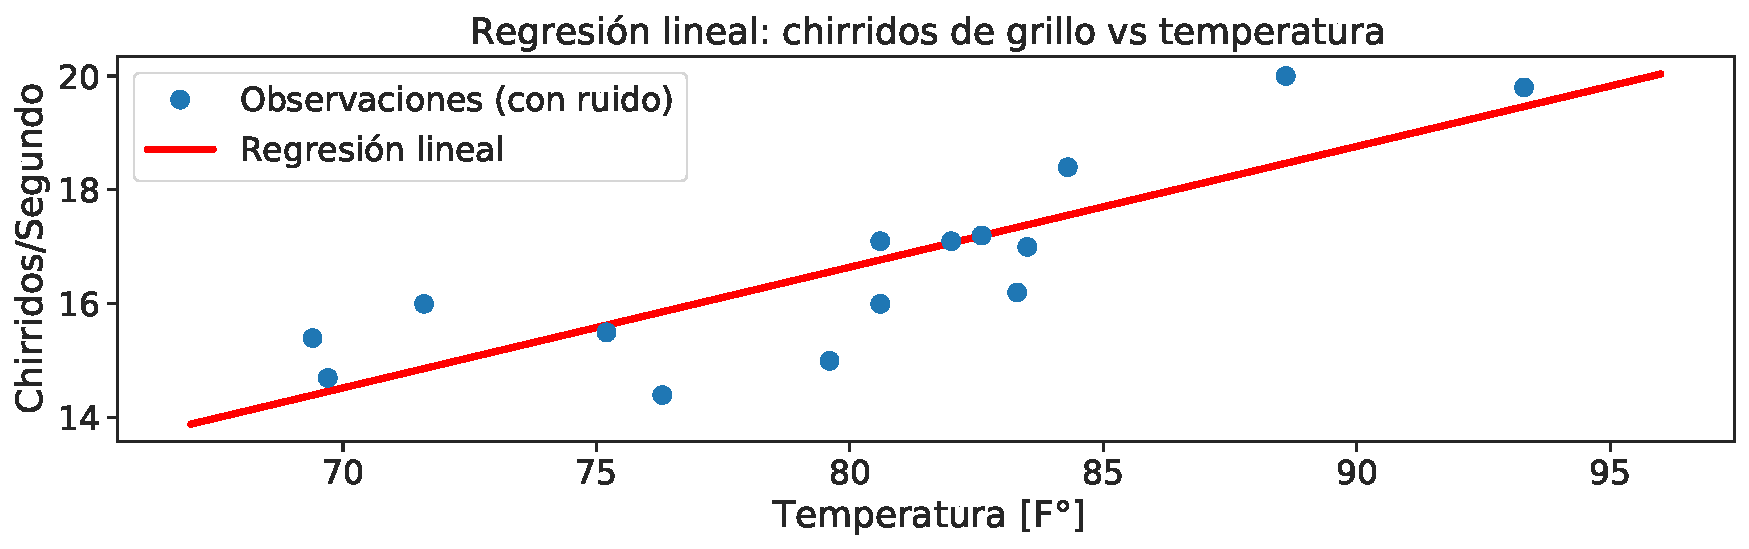
\includegraphics[width=0.9\textwidth]{img/cap1_chirridos.pdf}\\
	\caption{Ejemplo de regresión lineal mediante mínimos cuadrados sobre la base de datos de chirridos versus temperatura.}
	\label{fig:reg_lin_1}
\end{figure}

La expresión $\left(\tX^\top\tX \right)^{-1} \tX^\top$ en la ec.~\eqref{eq:sol_mse} corresponde a la pseudoinversa de Moore-Penrose de $\tX$ \cite[p.~7]{benisrael_greville_2006} y por lo tanto, es necesario que $r(\tX)=M+1$ (ver anexo). Además, dado que $\tX\in\R^{N\times (M+1)}$ entonces $r(\tX)\leq\min\{N,M+1\}$ por lo que necesariamente se necesita que $N\geq M+1$, es decir, que el número de muestras sea mayor que el número de dimensiones. Intuitivamente esto se debe a que se necesitan $M+1$ puntos para fijar un hiperplano en $\R^{M+1}$.\\

Es claro que para el caso de variables continuas es muy poco usual que dos observaciones sean perfectamente colineales, sin embargo, en el caso de variables categóricas donde las observaciones son asignadas a un número finito de símbolos es probable que dos o más valores para la variable dependiente sean exactamente iguales. \\

En la práctica, generalmente tendremos más observaciones que parámetros al considerar un modelo lineal y éstas serán linealmente independientes. Sin embargo, es posible que las observaciones sean tal que la inversión de la matriz  $\tX^\top\tX$ sea numéricamente  inestable. Esto ocurre fundamentalmente en dos casos ilustrados en el siguiente recuadro.  

\begin{mdframed}[style=discusion, frametitle={\center ¿Matriz cuasi-singular o incorrectamente escalada?}]

Al tratar de invertir una matriz de forma computacional, probablemente hemos obtenido un mensaje de la forma \texttt{matrix is singular, close to singular or badly scaled}. Veremos dos ejemplos para entender de dónde viene esta advertencia. 

\noindent\textbf{Caso 1:} Consideremos la matriz 
\begin{equation}
	A = \left[ \begin{matrix}10^{50} & 1 \\  10^{50}  & 2\end{matrix}\right]
\end{equation}
dicha matriz es claramente invertible y su inversa puede ser calculada mediante
\begin{equation}
	A^{-1} = \frac{1}{10^{50} \cdot 2 - 10^{50}\cdot 1}\left[ \begin{matrix}2 & -1 \\  -10^{50}  & 10^{50}\end{matrix}\right]
	=\left[ \begin{matrix}2\cdot10^{-50} & -10^{-50} \\  -1  & 1\end{matrix}\right],
\end{equation}
donde cuyos elementos difieren en 50 órdenes de magnitud. Sin embargo, la representación usual que consideramos cuando programamos es la de punto flotante de precisión simple, la cual considera el menor valor (de magnitud mayor que cero) de $2^{-127}\approx 10^{-38}$. Consecuentemente, los valores más pequeños que este límite serán aproximados por el elemento más cercano, es decir, cero. Utilizando la inversa aproximada, denotada $\tilde{A}^{-1}$, resulta en errores como el siguiente:
\begin{equation}
	A\tilde{A}^{-1} = \left[ \begin{matrix}10^{50} & 1 \\  10^{50}  & 2\end{matrix}\right] \left[ \begin{matrix} 0 & 0 \\  -1  & 1\end{matrix}\right] = \left[ \begin{matrix} -1 & 1 \\  -2  & 2\end{matrix}\right] \neq \eye
\end{equation}

\noindent\textbf{Caso 2:} Consideremos
\begin{equation}
	A = \left[ \begin{matrix} a  & a \\  b  & b + \epsilon\end{matrix}\right]
\end{equation}
la cual también es invertible para $a,\epsilon>0$, pues su determinante está dado por
\begin{equation}
	\det{A} = a(b+\epsilon) - ab = a\epsilon>0,
\end{equation}
sin embargo, si $\epsilon\ll1$ entonces el cálculo de la inversa puede sufrir inestabilidades numéricas como en el caso anterior. Sin embargo, observe para un $\eta>0$ suficientemente grande, la matriz $A+\eta I$ puede tener un determinante arbitrariamente grande (ver Sección \ref{sub:min_cuad_reg}).
\end{mdframed}

Es relevante reflexionar por qué consideramos mínimos cuadrados como la métrica de error relacionada al problema de regresión. Existen varias razones por que lo hacemos, tanto técnicas como conceptuales, como también diversas desventajas de este criterio que es importante identificar.  Desde del punto de vista técnico, el costo estrictamente convexo de un modelo lineal (en los parámetros) define un problema de optimización que también es estrictamente convexo y por ende tiene una solución única. Además, en el caso particular del costo cuadrático, este óptimo puede ser determinado de forma explícita (lo cual es fuertemente deseado), pues está dado únicamente por la inversión de una matriz y no mediante, e.g., una búsqueda iterativa.\\

Desde un punto interpretativo, el exponente 2 busca penalizar mayormente grandes diferencias (mayores que 1) entre predicción y valor real mientras que le quita importancia a errores de predicción pequeños (menores que 1). Si bien es posible utilizar otros exponentes bajo el mismo razonamiento de penalización, se utiliza mayormente la minimización de cuadrados ya que tiene propiedades matemáticas muy favorables en cuanto al análisis técnico por lo permite obtener conclusiones teóricas más fuertes.\\

Desde un punto de vista conceptual, otra justificación para usar la medida del  error cuadrático es que éste representa la varianza muestral. Es decir, si considerásemos que $x_i$ e $y_i$ son observaciones iid de variables aleatorias (VAs) $x$ e $y$ respectivamente, entonces el error cuadrático medio (relacionado con la función $f$) definido por
\begin{equation}
	e= \frac{1}{N-1}\sum_{i=1}^N (y_i-f(x_i))^2,
\end{equation}
es la varianza muestral de la variable aleatoria $y-f(x)$ (asumiendo que $\E(y-f(x))=0$). De igual forma, la varianza de la suma de múltiples variables aleatorias (pensemos en errores acumulados, los cuales son independientes) corresponde a la suma de las varianzas de dichas VAs. Esto ocurre precisamente cuando usamos el exponente igual a 2, y no si usáramos 1.95 o 2.05.\\

Podemos además justificar el uso del error cuadrático con una motivación geométrica. Recordemos que el problema de regresión (lineal) requiere encontrar una solución aproximada de un sistema lineal sobredeterminado definido por 
\begin{equation}
	\tX \theta = Y,\label{eq:sist_lineal_sobredet}
\end{equation}
donde la cantidad de incógnitas ($M+1$) es ampliamente superada por el número de ecuaciones ($N$). Como esta solución, desde el punto de vista de un sistema lineal, no necesariamente existe (y en la práctica no existe), uno puede proceder a encontrar la solución para $\theta$ que reporta \emph{la menor discrepancia} entre ambos lados de la ec.~\eqref{eq:sist_lineal_sobredet}. En este sentido, podemos identificar el espacio formado por todos los posibles valores que toma la combinación lineal $\tX \theta$ para distintos valores de $\theta\in\R^{M+1}$, es decir, el \emph{span} de todas las columnas de $\tX$, formando un subespacio vectorial estricto de $\R^N$. Luego, podemos identificar el elemento de dicho espacio que está más cerca de $Y\in\R^N$  como la proyección del propio $Y$ en $\text{span}(\tX)$. Esto está ilustrado en la Fig.~\ref{fig:projection}, donde la condición para identificar dicha proyección es  precisamente que el vector error $Y-\tX \theta$ sea ortogonal al espacio  $\text{span}(\tX)$ generado por los datos de entrada. Además, dado que las columnas de $\tX$ son una base de $\text{span}(\tX)$:

\begin{equation}
	u\in \text{span}(\tX) \iff \exists \theta_u\in \R^{M+1}: u=\tX\theta_u
\end{equation}

Por lo tanto:
\begin{equation}
	e\perp \text{span}(\tX) \iff e\perp u,\forall u \in \text{span}(\tX) \iff (Y-\tX \theta)^\top \tX \theta_u = 0, \forall \theta_u \in \R^{M+1} \iff (Y-\tX \theta)^\top \tX=0
\end{equation}
De lo anterior se recupera la solución de mínimos cuadrados:
\begin{equation}
	(Y-\tX \theta)^\top \tX = 0 \iff Y^\top \tX - \theta^\top \tX^\top \tX = 0 \iff \theta^\top = Y^\top \tX(\tX^\top \tX)^{-1} \iff \theta = (\tX^\top \tX)^{-1}\tX^\top Y
\end{equation}
\begin{figure}[t]
	\centering
	\includegraphics[width=0.45\textwidth]{img/LinRegGeo.pdf}\\
	\caption{Interpretación geométrica de la regresión lineal y mínimos cuadrados}
	\label{fig:projection}
\end{figure}
Finalmente, notemos que el criterio de  mínimos cuadrados (MC) también tiene desventajas. Implícitamente, MC está intrínsecamente relacionado con un supuesto de gaussianidad de los datos --- esto será evidente cuando estudiemos el criterio de máxima verosimilitud --- consecuentemente, el uso de MC produce estimaciones razonables cuando la relación entre $x$  e $y$ es simétrica y sin \emph{grandes desviaciones}. Por el contrario, cuando existen datos que se alejan mucho de la tendencia buscada, las estimaciones encontradas mediante MC pueden desviarse considerablemente de la solución buscada, esto se debe precisamente a la contribución cuadrática del error, donde, coloquialmente, una muestra \emph{muy alejada} pesa tanto o más que varias muestras \emph{ligeramente alejadas}. La Fig.~\ref{fig:reg_lin_2} ilustra este fenómeno para el mismo ejemplo de los chirridos en la Fig.~\ref{fig:reg_lin_1}, donde se ha introducido un \emph{outlier}, es decir, una observación que está inusualmente alejada de los datos y se ha recalculado el resultado de la regresión lineal mediante el criterio de MC. Se puede ver cómo se deteriora la estimación solo con la introducción de un nuevo dato. 

\begin{figure}[H]
	\centering
	\includegraphics[width=0.8\textwidth]{img/cap1_chirridos_outlier.pdf}\\
	\caption{Efecto de un \emph{outlier} en la regresión lineal usando mínimos cuadrados: Se ha agregado un dato erróneo (\emph{outlier} en gris) y se ha recalculado la regresión lineal, note cómo la inclusión de dicho punto deteriora el resultado de la regresión.}
	\label{fig:reg_lin_2}
\end{figure}

La lección que queda de este ejemplo es que debemos considerar una métrica \emph{ad hoc} al problema que estamos considerando, por ejemplo, si es muy probable que existan outliers, no debemos penalizar cuadráticamente los errores. De igual forma, al elegir una métrica de error debemos verificar cuán relevante es que el error de regresión sea i) nulo vs muy pequeño, o bien ii) grande vs extremadamente grande. La Fig.~\ref{fig:reg_lin_err} presenta cuatro métricas de error (como función del propio error), donde podemos interpretar sus propiedades. 

\begin{figure}[H]
	\centering
	\includegraphics[width=0.8\textwidth]{img/cap1_errores.pdf}\\
	\caption{Distintas funciones de costo en función del error de estimación, de izquierda a derecha: cuadrático, absoluto (crecimiento lineal en función del error), $\epsilon$-insensible (es irrelevante si el error está entre 0 o  $\epsilon$) y acotado (es irrelevante si el error es mayor que cierto umbral).}
	\label{fig:reg_lin_err}  
\end{figure}


\subsubsection{Regularización: ajuste versus generalización}
\label{sub:min_cuad_reg}

Perseguir ciegamente la solución de mínimos cuadrados puede resultar, como discutimos en la sección anterior, en situaciones donde la inversa de Moore-Penrose sea \emph{cercana} a singular, especialmente en los casos que las observaciones son parecidas o redundantes. En este sentido, debemos considerar un criterio que no simplemente busque un ajuste a los datos, sino que también promueva ciertas propiedades de la solución, por ejemplo, suavidad, bajas magnitudes de los parámetros o incluso pocos parámetros. Nos referiremos a estas soluciones como \emph{regulares}, y el objetivo de este apartado será \emph{regularizar} la solución de mínimos cuadrados.

Las penalizaciones a considerar en el problema de regresión pueden ser codificadas directamente en la función de costo. Por ejemplo, ésta puede incluir un término que promueve el ajuste de los datos y otro término que sanciona soluciones que se alejan de lo deseado. Un criterio estándar de penalización es el basado en la norma de los parámetros, es decir, 
\begin{equation}
	J_\rho = \norm{Y-\tX\theta}_2^2 + \rho\norm{\theta}_p^p,\ p\geq 0,
	\label{eq:reg_least_squares}
\end{equation} 
donde $||\cdot||_p$ denota la norma $\ell_p$, es decir, $||\theta||_p=\left(\sum_{j=1}^{M+1}|\theta_j|^p\right)^\frac{1}{p}$ y el parámetro $\rho\geq0$ tiene el rol de balancear la importancia entre ajuste (primer término) y regularidad de la solución (segundo término). Distintos valores de $p$ inducen distintos propiedades sobre las soluciones, siendo las más usadas las correspondientes a $p=1$, conocido como \textbf{LASSO}\footnote{\emph{Least Absolute Shrinkage and Selection Operator.}} \cite{tibshirani_1996}, y $p=2$ conocido como \textbf{regularización de Tikhonov\footnote{La regularización de Tikhonov puede ser generalizada mediante penalizaciones matriciales, de este modo se tiene un costo $J_\Gamma(\theta)=\norm{Y-\tX\theta}_2^2 + \norm{\Gamma\theta}_2^2  \implies \theta = \left(\tX^\top\tX +\Gamma^\top\Gamma\right)^{-1} \tX^\top Y$. Se recupera la regularización $L_2$ tomando $\Gamma = \alpha\eye$.}} \cite{tikhonov_arsenin_1977} o bien \textbf{\emph{Ridge Regression}}.\\  

Una ventaja de la regularización de Tikhonov es que su solución, al igual que el caso de mínimos cuadrados no regularizados, puede ser encontrada en forma exacta, en efecto, dado que el problema nuevamente es convexo:
\begin{align}
	&\nabla_\theta J_\rho = 0\\
	&\iff -2(Y-\tX\theta)^\top\tX + 2\rho\theta^\top =0\\
	&\iff -Y^\top\tX +\theta^\top\tX^\top\tX + \rho\theta^\top= 0\\
	&\iff \theta^\top = Y^\top \tX(\tX^\top\tX + \rho\eye)^{-1}\\
	&\iff \theta = (\tX^\top\tX+\rho\eye)^{-1}\tX^\top Y
\end{align}

De la última expresión, es posible ver que el requerimiento de que las observaciones disponibles sean (i) más que la dimensión $M+1$ y que además (ii) éstas sean colineales ya no es necesario para que la solución esté bien definida. De hecho, la matriz $\tX^\top\tX$ puede efectivamente estar cercana a ser no invertible, sin embargo, es posible \emph{regularizar} la solución forzando que la matriz $\left(\tX^\top\tX +\rho \eye\right)$ sea arbitrariamente lejana de las matrices singulares (o tenga un determinante arbitrariamente grande) aumentando el valor de $\rho$, en efecto:

\begin{lemma}
	Sea $A\in\mathcal{M}_{nn}(\R)$, entonces $\det(A+\rho\eye)\to \infty$ cuando $\rho\to\infty$.
\end{lemma}

\begin{proof}
	Para una matriz $M$ fija, $M^{ij}$ representará la matriz $M$ sin la fila $i$ ni la columna $j$. De este modo se tiene que:
	\begin{equation}
		\det(A+\rho\eye) = \sum_{i=1}^n (A+\rho\eye)_{1i}\cdot \det\left((A+\rho\eye)^{1i}\right) = p\cdot\det\left((A+\rho\eye)^{11}\right) + \sum_{i=1}^n a_{1i}\cdot \det\left((A+\rho\eye)^{1i}\right)
	\end{equation}
	
	Además, en el caso base ($n=1$), $\det(A+\rho\eye)=a+\rho\to\infty$ cuando $\rho\to\infty$. Dado que el determinante es un polinomio en $\rho$ de grado menor o igual a la dimensión de la matriz, entonces en el límite el primer sumando dominará a la sumatoria (ya que está multiplicado por $p$). De este modo, $\det(A+\rho\eye)\to \infty$ cuando $\rho\to\infty$.
\end{proof}


Es relevante entender por qué una disminución en la norma de los parámetros, puede ayudar a ajustar \emph{mejores} modelos. A primera impresión, un podría pensar que el criterio de mínimos cuadrados regularizados (MCR) en ningún caso puede reportar mejores modelos que su contraparte MC, pues MCR es una variante restringida del problema original y consecuentemente solo puede \emph{en el mejor de los casos} alcanzar la solución óptima. Esto es cierto si por \emph{mejor modelo} solo consideramos el error cuadrático medio (ECM), sin embargo, solo enfocarse en esta métrica no siempre es el mejor opción. Para ilustrar este concepto, tomemos las siguientes consideraciones: asumamos que efectivamente los datos cumplen la relación
\begin{equation}
	y_i = \underbrace{\theta^\top\tx_i}_{f_i} + \epsilon_i,	
 \end{equation}
 donde $\epsilon_i$ son observaciones iid de una variable aleatoria de varianza $\sigma^2$, $\theta$ es un parámetro fijo pero desconocido, los $\tx_i$ son fijos y $f_i= \theta^\top\tx_i$ se refiere a la  \emph{parte determinista} del modelo. Además, consideremos una estimación del parámetro $\theta$ construida en base a un conjunto de entrenamiento $D=\{(\tx_i,y_i)\}_{i=1}^N$, denotada $\hat\theta=\hat\theta_D$. Con estas consideraciones, se puede probar que para un nuevo par $(\tx_\star,y_\star)$, el \emph{error cuadrático esperado} asociado a la \textbf{predicción} $\hat f_\star = \hat\theta^\top \tx_\star$ se puede descomponer de acuerdo al trade-off entre el sesgo y la varianza \cite{ISLbook}. Dicha descomposición viene dada por:
 
\begin{equation}
 	\E{(y_\star - \hat f_\star)^2} = \text{Sesgo}(\hat f_\star)^2 + \text{Varianza}(\hat f_\star) + \sigma^2,\label{eq:expected_sq_loss}
 \end{equation} 

 donde el valor esperado es tomado con respecto a la ley de $\epsilon$, la única fuente de incertidumbre en este escenario. Los 3 sumandos de la descomposición corresponden a:
 \begin{itemize}
 	\item $\text{Sesgo}(\hat f_\star) := \E(\hat f_\star) - f_\star$. Representa una medida de exactitud: ¿cuán buena (en valor esperado) es la estimación con respecto al valor real?
 	\item $\text{Varianza}(\hat f_\star) = \E(\E(\hat f_\star)- \hat f_\star)^2$. Representa una medida de precisión: ¿cuán disperso es el estimador?
 	\item $\sigma^2$ es la varianza de \emph{ruido} $\epsilon$ y es la parte irreducible del costo, en el sentido que no puede ser controlada por la elección de $\hat\theta$.
 \end{itemize}

Podemos evaluar el sesgo y la varianza para el estimador de mínimos cuadrados, denotado $\hat\theta_{MC}$, eligiendo $\hat f_\star = \hat\theta_{MC}^\top\tx_\star$. En efecto, se tiene lo siguiente:

\begin{theorem} Bajo la hipótesis de ruido aditivo sobre un modelo lineal, el estimador de mínimos cuadrados cumple que:
	\begin{align}
	\text{Sesgo}(\hat f_\star) &= 0\\
	\text{Varianza}(\hat f_\star) &= \sigma^2 \tx_\star^\top (\tX^\top\tX)^{-1}	\tx_\star
\end{align}
\end{theorem}

Es decir, el modelo de regresión lineal ajustado mediante MC reporta un estimador insesgado (sesgo nulo) pero con una varianza que depende de los datos en el conjunto de entrenamiento $D$, la varianza del ruido $\sigma^2$ y la propia entrada $\tx_\star$. Si bien no es posible determinar cuánto es esta varianza sin tomar supuestos estadísticos sobre los $\tx_i$'s, recordemos que la matriz $\tX^\top\tX$ puede ser cercana a singular cuando los datos son pocos, redundantes o colineales, lo cual resultará en alta varianza para la predicción $\hat f_\star$. De hecho, si asumiéramos que $\tx_i\sim\cN(0,1)$ iid, tendríamos que $\text{Varianza}(\hat f_\star) = \sigma^2 M/N$, es decir, la varianza es inversamente proporcional a la razón entre la dimensión de las entradas ($M$) y la cantidad de muestras ($N$).

\begin{mdframed}[style=discusion, frametitle={\center Evaluaciones \emph{dentro de muestra} y \emph{fuera de muestra}}]
 Notemos que la expresión en la ec.~\eqref{eq:expected_sq_loss} es una medida de error \emph{fuera de muestra}, pues evalúa un estimador $\hat\theta$, construido en base a un conjunto $D$, en un nuevo dato $(\tx_\star,y_\star)$ que no está originalmente contenido en $D$. No debemos confundir esta expresión con el error cuadrático medio, en la ec.~\eqref{eq:least_squares_cost}, el cual representa un error \emph{dentro de muestra}. La  evaluación de ambos tipos de  costos es clave para diseñar modelos y estimadores que puedan \emph{generalizar} a datos no vistos. 
\end{mdframed}

Al penalizar la norma cuadrada del parámetro $\theta$, la regresión de Ridge sacrifica la propiedad insesgada del estimador de mínimos cuadrados, pero en retorno construye un estimador que tiene menos varianza que el de MC. Esto puede entenderse como el balance entre: i) confiar únicamente en los datos, los cuales pueden ser pocos o muy ruidoso y consecuentemente insuficientes para determinar un modelo apropiado, y ii) introducir un \emph{sesgo} al modelo (por ejemplo, parámetros pequeños) con la finalidad de robustecer el modelo encontrado en función de los datos disponibles. En efecto, se tiene lo siguiente:

\begin{theorem} Bajo la hipótesis de ruido aditivo sobre un modelo lineal, el estimador de mínimos cuadrados regularizados cumple que:
	\begin{align}
	\text{Sesgo}(\hat f_\star) & = \tx_\star^\top \left[(\eye+\rho(\tX^\top\tX)^{-1})^{-1}-\eye\right]\theta\\
	\text{Varianza}(\hat f_\star) &= \sigma^2 \tx_\star^\top (\tX^\top\tX + \rho\eye)^{-1}\tX^\top\tX(\tX^\top\tX+\rho\eye)^{-1}	\tx_\star
\end{align}

Además, la varianza de MCR es menor a la varianza de MC.
\end{theorem}

Esta noción de (sobre-)ajustar a los datos de entrenamiento versus generalizar a  nuevos  puede ser ilustrada con el siguiente ejemplo: Consideremos $N=1000$ datos relacionados linealmente (pares de entrada y salida) donde la dimensión de entrada es $M=100$, generados por el siguiente script:

\begin{lstlisting}[language=Python]
##generacion de datos relacionados linealmente.
n_samples, n_features = 1000, 100
rng = np.random.RandomState(0)
X = rng.randn(n_samples, n_features)
theta = rng.randn(n_features,1)
y = X@theta + 10rng.randn(n_samples, 1)
\end{lstlisting}

 En vez de utilizar todas las muestras de entrenamiento, utilicemos solo $N'=15$ muestras para entrenar usando los criterios de MC, y regresión de Ridge (RR) con $\rho\in\{40,80\}$. Repitiendo este proceso 400 veces, podemos analizar cómo se comportan los distintos métodos en cuanto a la magnitud de los parámetros encontrados, el error dentro de muestra (con respecto a los datos de entrenamiento) y el error fuera de muestra (con respecto a los datos no usados para entrenar). La Fig.~\ref{fig:MCvsRR_Synth} muestra dichos histogramas, desde donde podemos ver que a mayor $\rho$ (recordemos que MC es equivalente a RR con $\rho=0$), los parámetros encontrados tienen menor magnitud. Adicionalmente, notemos que el modelo no regularizado (MC) se comporta mejor en evaluación dentro de muestra, sin embargo, sus papeles se invierten cuando se trata de evaluación fuera de muestra: el incluir un sesgo en el ajuste de modelos (RR) puede ayudar a generalizar y no sobreajustar cuando se tienen pocos datos. 

 \begin{figure}[H]
	\centering
	\includegraphics[width=0.8\textwidth]{img/cap1_bias-variance.pdf}\\
	\caption{Mínimos cuadrados versus regresión de Ridge ($\rho\in\{40,80\}$): determinación de parámetros usando solo 15 muestras para un parámetro de dimensión $M=100$. De derecha a izquierda podemos ver magnitud de los parámetros encontrados, error dentro de muestra y error fuera de muestra. Experimento repetido 400 veces.}
	\label{fig:MCvsRR_Synth}  
\end{figure}

Si bien el problema de mínimos cuadrados regularizados incluye en su función objetivo una penalización sobre la norma de $\theta$, el problema también puede ser visto como el problema de mínimos cuadrados original con una restricción adicional que fija la norma del parámetro. En efecto, dicho problema viene dado por:
\begin{align}
	\min_\theta & \norm{Y-\tX\theta}_2^2\label{eq:MC_restriccion}\\
	\text{s.a.} &\ ||\theta||_p^p = \tau,\nonumber
\end{align}
donde $\tau\geq0$ es una constante conocida. Sabemos que este problema puede ser resuelto en su forma dual mediante la formulación del lagrangiano dado por 
\begin{equation}
	L = \norm{Y-\tX\theta}_2^2 - \lambda \left(||\theta||_p^p - \tau\right),
\end{equation}
donde $\lambda$ es el multiplicador de Lagrange asociado al problema. Luego, las condiciones de primer orden necesarias para encontrar la solución del problema con restricciones en la ec.~\eqref{eq:MC_restriccion} están dadas por: 
\begin{align}
	\frac{\partial L}{\partial \theta} = 0 &\quad\Rightarrow\quad  \frac{\partial }{\partial \theta}\left(\norm{Y-\tX\theta}_2^2 - \lambda ||\theta||_p^p \right) = 0\\
	\frac{\partial L}{\partial \lambda} = 0 &\quad\Rightarrow\quad ||\theta||_p^p = \tau, \label{eq:dual_MCR2}
\end{align}
lo cual recupera la forma del problema de minimización de mínimos cuadrados regularizados. Enfatizamos esta relación en el siguiente recuadro. 

\begin{mdframed}[style=discusion, frametitle={\center Mínimos cuadrados regularizados: optimización con restricciones}]
Observemos que el problema de mínimos cuadrados regularizados, determinado por el costo en la ec.~\eqref{eq:reg_least_squares}, es equivalente al dual de un problema de optimización con restricciones en las ecs.~\eqref{eq:dual_MCR1}-\eqref{eq:dual_MCR2} para un $\lambda$ dado tal que $\lambda =-\rho$. Consecuentemente, como el valor óptimo de $\lambda$ depende del nivel de la restricción $\tau$, podemos aseverar que \textbf{para cualquier $\rho\geq0$, existe un $\tau\geq0$ tal que la minimización de \eqref{eq:reg_least_squares} es equivalente a la de \eqref{eq:MC_restriccion}.} Consecuentemente,  podemos interpretar el problema de MCR como el de MC sujeto a una restricción sobre la norma del parámetro. 
	
\end{mdframed}

Con la interpretación del problema de optimización con restricciones sobre la norma del parámetro $\theta$, podemos entender distintos regularizadores (distintos $p\geq0$) mediante sus curvas de nivel. La Fig.~\ref{fig:reg_lin_reg} ilustra las curvas correspondientes al costo cuadrático (izquierda) y al término de regularización en la eq.~\eqref{eq:reg_least_squares} para órdenes $p\in\{0.5,1,2\}$. 

\begin{figure}[H]
	\centering
	\includegraphics[width=0.8\textwidth]{img/cap1_regularizadores.pdf}\\
	\caption{Curvas de nivel del costo cuadrático para un problema hipotético con solución $\theta=[10,20]$ (izquierda) y términos de regularización para órdenes $p\in\{0.5,1,2\}$. Observe cómo las curvas de nivel atraen el mínimo hacia el origen de distinta forma: $p=2$ lleva la solución directamente al origen, mientras que $p\in\{0.5,1\}$ lleva la solución a los bordes, es  decir, privilegiando soluciones ralas. La solución $\theta=[10,20]$ se ha denotado con una cruz azul, recuerde que solo el costo cuadrático depende de este valor, no los términos de regularización. }
	\label{fig:reg_lin_reg}  
\end{figure}

La formulación en base a restricciones es clave para entender la propiedad de \emph{selección de características} de los MCR. Al estimar el parámetro $\theta$, estamos verificando cuán importante es cada coordenada de la entrada o en la jerga de reconocimiento de patrones, cada \emph{característica}. Indirectamente estamos también implícitamente descubriendo cuáles son las características que importan y cuales no, a esto nos referimos como selección de características. Distintas normas para el término de regularización, como las ilustradas en la Fig.~\ref{fig:reg_lin_reg}, inducen distintas propiedades para la solución del problema de MCR. En particular, RR atrae \emph{homogéneamente} el parámetro hacia el origen, lo cual resulta  en estimaciones de menor varianza como vimos en el apartado anterior. LASSO ($p=1$) y el caso $p\leq1$ en general presenta una propiedad adicional, donde la forma de la curva de nivel permite que usualmente la solución del problema se concentre el las puntas del \emph{diamante} (ver Fig.~\ref{fig:reg_lin_reg}, $p=1$), llevando algunas coordenadas del parámetro $\theta$ directamente a cero. Por esto decimos que LASSO (y $p\leq1$ en general) tiene la propiedad de selección de variables y entrega modelos ralos con respecto a MC tradicional. 



Para ilustrar la propiedad de selección de características, consideremos el \emph{Breast Cancer Wisconsin Data Set}\footnote{\url{https://archive.ics.uci.edu/ml/datasets/breast+cancer+wisconsin+(original)}}, el cual tiene $N=569$ muestras y un dimensión de entrada de $M=30$. Los valores para la variable de salida ($y$) son solo dos, pues este es un problema de clasificación (\emph{cáncer} vs \emph{no-cáncer}), sin embargo, nosotros ajustaremos un modelo de regresión lineal usando MC, RR y LASSO para luego evaluar los pesos encontrados. Usaremos 2/3 de los datos para entrenar y el 1/3 restante para calcular puntajes fuera de muestra. La Fig.~\ref{fig:MC_RR_LASSO_breastcancer} presenta los parámetros encontrados para cada uno de los métodos, donde podemos ver la propiedad de selección de variables de LASSO; adicionalmente, la Tabla 1 muestra los puntajes de cada método, tanto dentro como fuera de muestras: en la línea de la discusión anterior, los modelos regularizados presentan mejor generalización y usan menos parámetros (o más parámetros iguales a cero). 

\begin{figure}[H]
	\centering
	\includegraphics[width=0.8\textwidth]{img/cap1_OLS_RR_LASSO.pdf}\\
	\caption{Parámetros de la regresión lineal del \emph{Breast Cancer Dataset} usando MC, RR y LASSO. Observe cómo RR y LASSO disminuye críticamente la magnitud de los parámetros y, además, LASSO lleva parámetros directamente a cero, resultando en un modelo más simple (i.e, con menos parámetros).}
	\label{fig:MC_RR_LASSO_breastcancer}  
\end{figure}

\begin{table}[h]
\centering
	\label{tab:breastMC_RR_LASSO}
	\begin{tabular}{ r|c|c } 
		 & in-sample & out-of-sample \\
		\hline
		MC & \textbf{0.7896} & 0.6911 \\ 
		RR & 0.6905 & 0.6903 \\ 
		LASSO & 0.7452 & \textbf{0.7242}
	\end{tabular}
	\caption{Puntajes de modelos de regresión implementados en \emph{Breast Cancer Wisconsin Data Set}, más alto es mejor. Observe la superioridad de los modelos regularizados para generalizar.}
\end{table}

Por otro lado, a pesar de que LASSO es un problema convexo, no es estrictamente convexo por lo que el regresor óptimo puede no ser único. Además, a diferencia de ridge-regression, LASSO no tiene una solución con forma cerrada por lo que se debe optimizar con algoritmos de programación cuadrática. Otra de las desventajas que tiene este regularizador ocurre al trabajar con entradas de alta dimensión (por ejemplo, imágenes o videos) y un conjunto de entrenamiento pequeño (es decir, $N< M$), donde la selección de características escoge a lo más $N$ componentes no nulas y el resto las descarta, ignorando posibles correlaciones entre las variables debido a un conjunto de entrenamiento pequeño. Para evitar esto, se pueden utilizar la regularización LASSO y ridge al mismo tiempo, resultando en lo que se denomina elastic net regularization, cuya función de costos es:

\begin{equation}
	J_\rho = \norm{Y-\tX\theta}_2^2 + \lambda_1\norm{\theta}_2^2 + \lambda_2\norm{\theta}_1
	\label{eq:reg_least_squares}
\end{equation} 

La introducción de un regularizador cuadrático fuerza a que la función de costos sea estrictamente convexa, por lo que el problema de minimización ahora tiene solución única.

\begin{mdframed}[style=discusion, frametitle={\center Consideraciones generales}]

Para concluir esta sección, es importante tener en cuenta las siguientes  consideraciones generales acerca de MCR:\\

$\bullet$ \textbf{¿es justo comparar MC y MCR en términos del ECM?} Ciertamente no, el criterio de MC siempre reportará un menor ECM, pues ha sido entrenado para minimizar dicho costo. Las ventajas de MCR están en su desempeño fuera de muestra, selección de variables o en  general en su habilidad de  incorporar  sesgo  \emph{de diseñador} en la soluciones que no afloren naturalmente de  los  datos. \\

$\bullet$ \textbf{¿cómo elegir $\rho$?} De forma general, este \emph{hiperparámetro} determina el balance entre regularización (cuán  sesgado) y ajuste (cuán bien replica  los datos de entrenamiento), consecuentemente lo debemos elegir según nuestra intención. En la práctica, se puede evaluar el desempeño fuera de muestra para distintos valores de $\rho$ con la finalidad de elegir un valor apropiado. Una manera de realizar la evaluación de desempeño para diferentes $\rho$ es la \emph{validación cruzada} (ver selección de modelos).\\

$\bullet$ Vimos que la norma $\ell_p$ con $0<p\leq1$ tiene la propiedad de selección de características, pero, \textbf{¿qué pasa con la ``norma'' $\ell_0$?}. La cantidad  $\ell_0(\theta)$ denota la cantidad de elementos no nulos de $\theta$ y, si bien no es una norma en el sentido formal de la palabra, puede de todas formas ser usada en la definición del costo en la ecuación ~\eqref{eq:reg_least_squares}, con la finalidad de directamente penalizar la cantidad de características usadas por el modelo. Desafortunadamente, encontrar la solución usando la ``norma'' $l_0$ es muy difícil, sin embargo, bajo ciertas condiciones, la consideración de la norma $l_1$ puede llevar a la misma solución.
\end{mdframed}

\subsection{Máxima verosimilitud}
\label{sub:max_ver}

En el apartado anterior vimos que para la regresión lineal, el criterio de  mínimos cuadrados, y su variante regularizada, ofrecen una alternativa simple, elegante, interpretable y con solución en forma cerrada. Sin embargo, también vimos que dicho criterio sufre de desventajas en cuanto a su capacidad de ajustar modelos en casos generales, pues el criterio de MC es particularmente apropiado para variables continuas, con perturbaciones aditivas  y simétricamente dispersas con respecto a una tendencia dada. Existen distintos casos donde el criterio de MC no es apropiado, por ejemplo aplicaciones financieras con  perturbaciones multiplicativas, mediciones de intensidad como frecuencia de aparición de palabras o sismos en donde las perturbaciones son con alta probabilidad solo positivas, y problemas de clasificación o asignación (\emph{clustering}) en donde las métricas de error toman la forma como ``correcto''/``incorrecto'', con lo que una medida de error que que reporte ajustes ``más incorrectos'' no tiene sentido. \\

Una alternativa natural es considerar una métrica de desempeño distinta y diseñada específicamente en función  de cada aplicación con la finalidad de capturar asimetrías, no-estacionariedad, asignación correcta e invarianzas (en el problema de \emph{clustering} por ejemplo) entre otras propiedades. Sin embargo, esta no solo es una tarea tediosa y poco elegante---en el sentido que va en contra los objetivos de inteligencia artificial expuestos en el Capítulo~\ref{cap:intro}---sino que puede ser muchas veces impracticable, pues precisamente no conocemos cuáles son las propiedades de los datos antes de ajustar modelos. Además, usar distintas métricas dificulta la interpretación y comparación de los enfoques considerados. Consecuentemente, nos proponemos considerar un criterio global de ajuste de modelos, el que en cada caso particular \emph{colapse} a una forma explícita que sí es \emph{ad hoc} al problema/modelo en cuestión y permite comparar distintos enfoques de manera unificada.\\

El enfoque general para ajuste de modelos que consideraremos en esta sección, y continuaremos utilizando durante el resto del curso, será el \emph{criterio  de máxima verosimilitud}, dado un conjunto de datos de entrenamiento $D$. Este es un criterio general para una amplia gama de modelos que, tal como se mencionó en el párrafo anterior, toma una  forma específica en cada problema, aunque su solución no siempre es calculable de forma explícita. Este enfoque es radicalmente distinto al de MC y a cualquier otro criterio de ``ajuste'': con el criterio MC se asume que ningún modelo es el modelo correcto y por lo tanto se busca un modelo \emph{aproximado} a los datos tal que la discrepancia entre el modelo candidato y los datos sea mínima. Por el contrario, en el criterio de \emph{máxima verosimilitud} nuestro objetivo es encontrar el modelo que---con mayor probabilidad---ha generado \emph{exactamente} los datos observados. Debido a la naturaleza aleatoria de los datos, para implementar este concepto es necesario considerar modelos probabilísticos, de forma de poder calcular la probabilidad de que los datos $D$ hayan sido generados por un modelo $m$, luego, elegiremos  el modelo que maximice dicha probabilidad. \\

El criterio de máxima verosimilitud (MV) es aplicable a modelos probabilísticos para la generación de datos, a los cuales nos referiremos como \emph{modelo generativos}. Para el caso del problema de regresión, el modelo generativo es cualquiera que modele la variable de salida como una variable aleatoria $y$ a través de una distribución condicional (a la entrada $x$ y el parámetro $\theta$) de la forma 
\begin{equation}
	y|x,\theta \sim p(y|x,\theta),\label{eq:mod_gen}
\end{equation}
donde enfatizamos que $y$ es  la única variable aleatoria y tanto el parámetro $\theta$ como la entrada $x$ son cantidades fijas (la primera desconocida y la segunda conocida u observable).

\begin{mdframed}[style=discusion, frametitle={\center Notación sobre variables aleatorias}]
 Si bien la convención estándar en teoría de probabilidades es denotar las variables aleatorias con letras mayúsculas, en este apunte se seguirá la usanza de la comunidad de Aprendizaje de Máquinas donde denotamos la tanto la variable aleatoria como su valor indistintamente con la letra minúscula, e.g., $y$. Seguiremos esta notación a menos que sea estrictamente necesario para evitar confusión. Además, en todos los casos asumiremos que las distribuciones de probabilidad consideradas tienen densidad con respecto a alguna medida --- usualmente \emph{Lebesgue} (caso continuo) o \emph{cuenta-puntos} (caso discreto) --- en ambos casos denotadas indistintamente por $p(\cdot)$.  Finalmente, usualmente escribiremos 
  \begin{equation}
  	y|x \sim p(y|x),
  \end{equation}
  sin enunciar explícitamente la dependencia del parámetro $\theta$, esto con el fin de no sobrecargar la notación.
\end{mdframed}


En particular, en el caso de la regresión lineal podemos considerar el siguiente modelo  generativo:
\begin{equation}
	y = a^\top x + b + \epsilon,\quad \epsilon\sim\cN(0,\sigma_\epsilon^2),
	\label{eq:lin_gauss}
\end{equation}
el cual consta de una parte determinística (afín en $x$) y una parte aleatoria caracterizada por la variable aleatoria $\epsilon$, la cual hemos  elegido gaussiana con media cero y varianza $\sigma_\epsilon^2$ (por determinar). El modelo probabilístico en la ec.~\eqref{eq:lin_gauss} puede expresarse mediante la siguiente densidad condicional 
\begin{equation}
	y|x \sim p(y|x,\theta) = \cN(y;a^\top x + b ,\sigma_\epsilon^2),\label{eq:mod_lin_gau}
\end{equation}
donde hemos denotados el vector de todos los parámetros del modelo mediante $\theta = [a,b,\sigma_\epsilon^2]$.\\

Si bien, lo siguiente no es necesario en el caso general, usualmente asumiremos que las realizaciones del modelo anterior, i.e., los datos $\{y_i\}_{i=1}^N$ generados a partir de la entrada $\{x_i\}_{i=1}^N$, son \textbf{condicionalmente independientes} dado el modelo. Esto significa que \emph{si conociésemos el modelo}, o  equivalentemente, si conociésemos $\theta$, y dos entradas $x_i,x_j$ independientes, entonces las  salidas correspondientes $y_i,y_j$ son independientes. Es importante clarificar que los valores generados por el modelo $\{y_i\}_{i=1}^N$ \textbf{no son independientes}. En efecto, si fuesen independientes no podríamos hacer predicciones: la predicción de una observación nueva $y_\star$ en base a una secuencia de observaciones $\{y_i\}_{i=1}^N$ estaría dada por\footnote{Hemos ignorado la dependencia de las variables independientes $\{x_i\}_{i=1}^N$, $x_\star$.}
\begin{equation}
	\blueb{[esto es falso]}\qquad p(y_\star|\{y_i\}_{i=1}^N) 
	\stackrel{\text{(prob. cond.)}}{=} \frac{p(y_\star,\{y_i\}_{i=1}^N)} {p(\{y_i\}_{i=1}^N)} 
	\stackrel{\text{(indep.)}}{=} \frac{p(y_\star),p(\{y_i\}_{i=1}^N)} {p(\{y_i\}_{i=1}^N)}
	=p(y_\star), 
\end{equation}
es decir, las observaciones pasadas no aportarían para la predicción.  Por  el contrario, como nuestro supuesto es de \textbf{independencia condicional} la expresión correcta es  la siguiente: 
\begin{equation}
	\blueb{[esto es verdadero]} \qquad p(y_\star|\{y_i\}_{i=1}^N,\theta)  
	=p(y_\star|,\theta), \qquad  \qquad\qquad  \qquad \qquad  \qquad\qquad  \qquad
\end{equation}
lo cual quiere decir que las  observaciones pasadas no son útiles para predecir el  futuro \textbf{solo si conozco el modelo}. Esto es evidente, pues si conozco el modelo, no necesito datos para saber de $y_\star$. \\


El supuesto de independencia condicional está garantizado al imponer que las realizaciones de $\epsilon\sim\cN(0,\sigma_\epsilon^2)$ sean \emph{independientes e idénticamente distribuidas} (iid). Esto es  fundamental para poder aprender el modelo desde múltiples observaciones, pues intuitivamente todas las observaciones aportan evidencia no redundante sobre el parámetro en común $\theta$. Por el contrario, si las observaciones fuesen condicionalmente dependientes, entonces la información que reportan para estimar $\theta$ sería redundante. Igualmente, si no todas las observaciones siguiesen la misma distribución, entonces cada una tendría ``su propio $\theta$'' y solo tendríamos ``un  dato'' para estimar cada parámetro. Más adelante en el curso veremos casos donde los datos no son iid pero asumimos cierta regularidad en los modelos que permiten determinar sus parámetros.\\

La dependencia de las observaciones cuando el modelo es desconocido permite introducir la siguiente definición:

\begin{definition}[verosimilitud]
Consideremos un  modelo generativo definido mediante la densidad de  probabilidad  $y\sim p(y|\theta)$, donde $\theta\in\Theta$ es el parámetro (desconocido) del modelo. Sean además $\{y_i\}_{i=1}^N$ observaciones generadas por dicho modelo. Se define $L: \Theta \to [0,1]$ como la probabilidad de los datos observados condicional al parámetro $\theta$, es decir, 
\begin{equation}
			\theta   \mapsto L(\theta) :=  p(\{y_i\}_{i=1}^N | \theta),
\end{equation}
Dicho valor de $L$ se denomina \emph{verosimilitud} del modelo $p(y|\theta)$ o, equivalentemente, del  parámetro $\theta$. En algunos casos, consideraremos la  notación $L_\y(\theta)$ para enfatizar que la verosimilitud es tomada con respecto a las observaciones  $\y$.
\end{definition}

La definición anterior es elocuente: la función de verosimilitud precisamente cuantifica cuán verosímil es un modelo (o equivalentemente, un parámetro) de haber generado las observaciones $\{y_i\}_{i=1}^N$. En este sentido, ante dos valores candidatos para el parámetro, por ejemplo $\theta_1$ y $\theta_2$, éstos pueden se evaluados mediante la comparación de $L(\theta_1)$ y $L(\theta_2)$. En efecto, si la razón $L(\theta_1)/L(\theta_2)$ es, por ejemplo, 3, entonces diremos que \emph{el valor de $\theta$ sea $\theta_1$ es 3 veces más verosímil a que sea $\theta_2$}. En este sentido, la función de verosimilitud  $L(\theta)$ representa una medida relativa de la \emph{bondad} de cada valor que el parámetro pueda tomar en función de los datos observados.

Es importante enfatizar que la función $L(\theta)$ \textbf{no es una densidad de probabilidad}. En efecto, podemos considerar la siguiente función en dos variables: $\theta$ y $\y=\{y_i\}_{i=1}^N$   
\begin{equation}
	\tilde{L}(\theta,\y) = p(\y|\theta),
\end{equation}
la cual toma distintos significados si  fijamos una de las variables: Si fijamos el valor del parámetro $\theta$, entonces, $\tilde{L}(\theta,\cdot) = p(\cdot|\theta)$ es una densidad de probabilidad, en efecto: 
\begin{equation}
	\int_{\R^N}\tilde{L}(\cdot,\y)\td\y = \int_{\R^N}p(\y|\theta)\td\y = 1,
\end{equation}
lo que quiere decir que para ``cualquier $\theta$'', $p(\y|\theta)$ es un modelo válido. Por el contrario, si fijamos $\y$, entonces obtenemos la función de verosimilitud: $\tilde{L}(\cdot,\y) = p(\y|\cdot) = L_\y(\theta)$, la  cual no necesariamente integra uno con respecto a $\theta$.

\begin{mdframed}[style=ejemplo, frametitle={\center Ejemplo: Verosimilitud para el modelo gaussiano  (muestras  independientes)}]

Consideremos un  modelo gaussiano definido por 
\begin{equation}
	y \sim p(y|\mu,\sigma^2) = \frac{1}{\sqrt{2\pi\sigma^2}}\exp\left(\frac{-(y-\mu)^2}{2\sigma^2}\right), \label{eq:ejemplo_gaussiano}
\end{equation}
y las observaciones $\y = \{y_i\}_{i=1}^N$ iid. La verosimilitud  de $\theta  =  [\mu,\sigma^2]$ está dada por 
\begin{align}
  	L(\theta)  &=  p(\y|\mu,\sigma^2) \stackrel{\text{(iid)}}{=}\prod_{i=1}^N p(y_i|\mu,\sigma^2) = \prod_{i=1}^N \frac{1}{\sqrt{2\pi\sigma^2}}\exp\left(\frac{-(y_i-\mu)^2}{2\sigma^2}\right)\nonumber\\ 
  				 &= \frac{1}{(2\pi\sigma^2)^{N/2}}  \exp\left(\frac{-\sum_{i=1}^N(y_i-\mu)^2}{2\sigma^2}\right)\nonumber\\
  				  & = \frac{1}{(2\pi\sigma^2)^{N/2}} \exp\left(\frac{-\left(\sum_{i=1}^Ny_i^2 - 2\mu\sum_{i=1}^Ny_i + N\mu^2\right)}{2\sigma^2}\right)\nonumber\\
  				  & = \frac{1}{(2\pi\sigma^2)^{N/2}}  \exp\left(\frac{-N\left(\sum_{i=1}^Ny_i^2/N \sred{-(\sum_{i=1}^Ny_i/N)^2 +(\sum_{i=1}^Ny_i/N)^2}- 2\mu\sum_{i=1}^Ny_i/N + \mu^2\right)}{2\sigma^2}\right)\nonumber\\
  				  & = \frac{1}{(2\pi\sigma^2)^{N/2}}  \exp\left(\frac{-(\sum_{i=1}^Ny_i^2/N  - (\sum_{i=1}^Ny_i/N)^2)}{2\sigma^2/N}\right)\exp\left(\frac{-(\mu - \sum_{i=1}^Ny_i/N)^2}{2\sigma^2/N}\right)
  				\nonumber\\
  				  & = \frac{1}{(2\pi\sigma^2)^{N/2}}  \exp\left(\frac{-(\bar s  - \bar y^2)}{2\sigma^2/N}\right)\exp\left(\frac{-(\mu - \bar y)^2}{2\sigma^2/N}\right)
  				\nonumber,
  \end{align}  
  donde $\bar y = \tfrac{1}{N}\sum_{i=1}^Ny_i$ es el promedio de las observaciones y $\bar s = \sum_ {i=1}^Ny_i^2/N$ es el promedio de los cuadrados de las observaciones. Observemos que como funciones de $\mu$ y $\sigma^2$, la expresión anterior es respectivamente  proporcional a las densidades Normal (para $\mu$) y Gamma-inversa (para $\sigma^2$). Sin embargo, recordemos que esta  expresión no necesariamente integra uno y por  ende es solo coincidentemente proporcional a una pdf conocida. La Fig.~\ref{fig:gaussian_likelihood} muestra la  densidad normal ($\mu=0,\sigma=1$) y la verosimilitud para ambos parámetros con 20 y 200 muestras. 

\begin{figure}[H]
	\centering
	\includegraphics[width=0.8\textwidth, frame]{img/cap1_gaussian_likelihood}\\
	\caption{Densidad normal (izquierda, $\mu=0$ y $\sigma=1$) y verosimilitud para la media y la varianza en base a 20 (centro) y 200 (derecha) observaciones.}
	\label{fig:gaussian_likelihood}  
\end{figure}
  
\end{mdframed}

\subsubsection{Elección del modelo de acuerdo a la máxima verosimilitud}

La verosimilitud es fundamental cuando realizamos \emph{inferencia}, es decir, cuando nuestro objetivo es descubrir o identificar los modelos y parámetros en base a las observaciones que dicho modelo ha generado; esto muchas veces se refiere coloquialmente como \emph{probabilidad inversa}. La importancia de la función de verosimilitud está documentado en el \textbf{principio de la verosimilitud}, el cual sentencia que toda la información relevante que la observación $\y = \{y_i\}_{i=1}^N$ puede aportar a la estimación del parámetro $\theta$, está contenido en la función  de verosimilitud $L(\theta)$. Una consecuencia directa de este principio es que si diseñamos dos experimentos para realizar  inferencia  sobre un parámetro desconocido $\theta$ y ambos  resultan en la misma función de verosimilitud  (salvo una constante de proporcionalidad), entonces,  ambos experimentos, y los datos adquiridos en  ellos, reportan la misma  información  sobre $\theta$. Lo de igualdad salvo una constante de proporcionalidad es porque recordemos que la verosimilitud es una medida \emph{relativa} de la bondad de (cada valor del) parámetro a inferir. \\

La pregunta  natural entonces es ¿cómo usar la función $L_\y(\theta)$ para determinar ``el buen $\theta$''? Por supuesto el título de esta sección hace las veces de \emph{spoiler} para esta pregunta: simplemente elegir el máximo de la función, pues éste nos da el(los) valor(es) más \emph{verosímil} para $\theta$ relativo a todo el resto de las opciones disponibles. Sin embargo, veamos que el uso del argumento que maximiza $L_\y(\theta)$ tiene un significado  mucho más  acabado. Consideremos la siguiente forma de encontrar el parámetro $\theta$: recordemos que el  modelo real es $p(y|\theta)$ y definamos una discrepancia entre modelos, denotada $D(p_1,p_2)$, luego, encontraremos el $\hat\theta$ tal que $p(y|\hat\theta)$ es lo más \emph{cercano} posible al modelo real con respecto a la discrepancia $D(\cdot,\cdot)$, es decir, el que minimiza la expresión
\begin{equation}
    	D(p(y|\theta),p(y|\hat\theta)).
\end{equation}  
Este criterio es interesante, pues notemos que no hemos incorporado ningún supuesto sobre la parametrización de  los  modelos (cómo el  modelo depende de $\theta$) ni de la  geometría del espacio  $\Theta$; estamos comparando directamente los modelos y no los  valores específicos de los parámetros. Desafortunadamente, notemos que formular y resolver  este problema no es posible en el caso general, pues la expresión de arriba depende del parámetro real $\theta$, el cual no conocemos, con lo que no podríamos resolver dicho problema de optimización. 

Sin embargo, veamos que podemos considerar una métrica que ofrece una alternativa para optimizar la discrepancia entre el modelo real y el aproximado, independientemente de que no conozcamos el valor de $\theta$. Dicha métrica, la cual es motivada desde la teoría de la información, es un estándar para comparar distribuciones de probabilidad generales y es conocida como la divergencia de Kullback-Leibler (ver anexos). Bajo esta métrica, la discrepancia entre el modelo real $p =  p(y|\theta)$ y el aproximado $q  = p(y|\hat\theta)$ viene dada por:
\begin{equation}
 	\KL( p(y|\theta),p(y|\hat\theta)) =  \int_y\log\left(\frac{p(y|\theta)}{p(y|\hat\theta)}\right)p(y|\theta)\td y.\label{eq:KL_maxlike}
 \end{equation} 
 En general, no es claro que podamos calcular dicha integral, sin embargo, observemos que esta es una  esperanza con respecto a la densidad $p(y|\theta)$, por lo que podemos considerar su aproximación de Monte Carlo usando las $N$ observaciones en $D$, las cuales están precisamente generadas por la medida de la integral en la ec.~\eqref{eq:KL_maxlike} de acuerdo a 
\begin{equation}
	\KL( p(y|\theta),p(y|\hat\theta)) 	\approx \KL_N( p(y|\theta),p(y|\hat\theta)) = \frac{1}{N}\sum_{i=1}^N\log\left(\frac{p(y_i|\theta)}{p(y_i|\hat\theta)}\right).
\end{equation}

Denotemos ahora $\hat\theta_N$ el minimizante de la  expresión anterior, el cual podemos calcular mediante (ignoramos la constante $N^{-1}$)
 \begin{align}
 	\hat\theta_N & =  \argmin_{\hat\theta}  \sum_{i=1}^N\log\left(\frac{p(y_i|\theta)}{p(y_i|\hat\theta)}\right)\\
 				&= \argmin_{\hat\theta}  \sum_{i=1}^N  \log p(y_i|\theta) - \sum_{i=1}^N \log p(y_i|\hat\theta)\nonumber\\
 				&= \argmax_{\hat\theta}  \sum_{i=1}^N \log p(y_i|\hat\theta)\nonumber\\
 				&= \argmax_{\hat\theta}  \prod_{i=1}^N p(y_i|\hat\theta),\nonumber
 \end{align}
 donde hemos eliminado los términos que no dependen de $\hat\theta$ y se ha usado el hecho de que el logaritmo es estrictamente creciente. Observemos que si nuestras muestras son condicionalmente independientes, entonces la expresión anterior implica que $\hat\theta_N$ es también el maximizante de la función de verosimilitud:
 \begin{align}
 	\hat\theta_N &= \argmax_{\hat\theta}  \prod_{i=1}^N p(y_i|\hat\theta) = \argmax_{\hat\theta}  p(\y|\hat\theta) = \argmax_{\hat\theta}  L_\y(\theta),
 \end{align}
 al que nos  referiremos como \emph{estimador de máxima verosimilitud}. Finalmente, queda la pregunta de cómo se relaciona el estimador de máxima verosimilitud (MV) $\hat\theta_N$ con el estimador óptimo en el sentido KL, $\hat\theta$. Para esto, notemos que la aproximación de Monte Carlo de la KL en la ec.~\eqref{eq:KL_maxlike} converge puntualmente a la KL,  i.e., para cada $\theta\in\Theta$,  $\KL_N( p(y|\theta),p(y|\hat\theta))\to \KL( p(y|\theta),p(y|\hat\theta))$ por la ley de los grande números  cuando $N\to\infty$. Consecuentemente, podemos asumir que los minimizantes  de la secuencia de aproximaciones de Monte Carlo también convergen al minimizante de la KL. Esta es la razón por la cual consideramos el estimador de máxima verosimilitud: en el límite ($N\to \infty$), el estimador de MV es el que reporta la mínima divergencia (KL) entre  el modelo real y el aproximado. Esta condición nos da un sentido de \emph{consistencia} del estimador de MV, donde por consistencia entendemos que mientras más datos observamos nuestra aproximación del modelo converge al mejor modelo posible (en la métrica KL). \\

\subsubsection{Maxima verosimilitud del modelo lineal gaussiano}

Retomemos el problema  de regresión lineal: la verosimilitud del modelo lineal gaussiano  definido en la ec.~\eqref{eq:mod_lin_gau} (con parámetro $\theta  = [a,b,\sigma_\epsilon^2]$) está dada por (recordemos  que  los datos son condicionalmente independientes)
\begin{equation}
	L_\y(\theta) =  \prod_{i=1}^N \cN(y_i;a^\top x_i + b,\sigma_\epsilon^2) = \frac{1}{(2\pi\sigma_\epsilon^2)^{N/2}}  \exp\left(\frac{-\sum_{i=1}^N(y_i-a^\top x_i - b)^2}{2\sigma_\epsilon^2}\right). \label{eq:verosimilitud_lineal}
\end{equation} 
Usualmente, se usa el logaritmo de la verosimilitud, referido como \emph{log-verosimilitud}, $l(\theta) = \log L(\theta)$, por su facilidad de interpretación y optimización. Recordemos que esta transformación es válida, pues la función logaritmo es estrictamente monótona y consecuentemente el(los) mínimo(s) no cambia(n).  De este modo, la log-verosimilitud del modelo lineal y gaussiano está dada por
\begin{equation}
	l(\theta) 
		= \underbrace{-N\log \sqrt{2\pi\sigma^2_\epsilon}}_{\text{dispersión}} + \underbrace{\frac{-1}{2\sigma_\epsilon^2} \sum_{i=1}^N (y_i-a^\top x_i - b)^2}_{\text{ajuste}},
\end{equation}
donde podemos de inmediato reconocer que la maximización de $l(\theta)$ implica el balance entre dos términos. El de la izquierda es una medida de dispersión o complejidad, pues para aumentar éste termino necesitamos que la varianza sea pequeña o el modelo tenga errores poco dispersos. El término de la derecha, por otro lado, es una medida de ajuste, para aumentar éste término necesitamos que el modelo  represente bien, muestra a muestra, nuestros datos. 

En particular, el estimador  de máxima verosimilitud para los parámetros de  la parte lineal (i.e., ignorando $\sigma^2_\epsilon$) está dado por:
\begin{align}
	 [a^{\text{MV}} ,b^{\text{MV}} ]
						&= \argmin_{a,b} \sum_{i=1}^N (y_i-a^\top x_i - b)^2. \label{eq:theta_ML}
\end{align}
Para  nuestra  sorpresa, observemos que es posible identificar esta última expresión con la del costo de mínimos cuadrados, es decir, el estimador de máxima verosimilitud es el minimizante del mismo costo que el estimador de mínimos cuadrados. Consecuentemente, ambos estimadores son iguales y por lo tanto:
\begin{equation}
	 [\hat{a},\hat{b}] = [a^{\text{MV}} ,b^{\text{MV}} ]=[a^{\text{MC}} ,b^{\text{MC}} ] = \left(\tX^\top\tX\right)^{-1} \tX^\top Y.
\end{equation}

Además, recordemos que luego de determinar el estimador con criterio de MC, es posible calcular la varianza de los errores (error cuadrático medio) de nuestro modelo mediante 
\begin{equation}
	\text{Varianza} = \frac{1}{N}\sum_{i=1}^N (y_i-\hat{a}^\top x_i -\hat{b})^2,
\end{equation}

Por otra parte, en el contexto de máxima verosimilitud, recordemos que la varianza es un parámetro del modelo y no una cantidad asociada al modelo que calculamos de forma independiente. Este parámetro puede ser calculado maximizando la log-verosimilitud, tal como se hizo para la media en la ecuación \eqref{eq:theta_ML}, de acuerdo a
\begin{align}
	\sigma^2_{\text{MV}} &= \argmax -\frac{N}{2} \log(\sigma_\epsilon^{2}) + \frac{-1}{2\sigma_\epsilon^2}\sum_{i=1}^N {(y_i-a^\top x_i -b)^2}. \label{eq:sigma_ML}
\end{align}
Dado que ya se optimizó sobre los parámetros $a$ y $b$, solo falta aplicar  la condición de primer orden sobre $\sigma_\epsilon^2$:
\begin{align}
	\frac{\partial l(\theta)}{\partial \sigma_\epsilon^2} = -\frac{N}{2\sigma_\epsilon^2} + \frac{1}{2(\sigma^2_{\text{MV}})^2}\sum_{i=1}^N {(y_i-\hat{a}^\top x_i -\hat{b})^2} = 0 \Rightarrow \sigma_\epsilon^2 = \frac{1}{N}\sum_{i=1}^N {(y_i-\hat{a}^\top x_i -\hat{b})^2}.
\end{align}
Con lo cual se obtiene, sin sorpresa alguna, la misma expresión de la varianza que al usar mínimos cuadrados. Además, observemos que el estimador de MV de la varianza depende de los parámetros $a$ y $b$, pero no al revés.\\

En la práctica, consideraremos la minimización de la log-verosimilitud negativa (en vez de la maximización de la log-verosimilitud) en línea con la literatura y software dedicados a la minimización de funciones. 

\subsection{Regresión via inferencia bayesiana} 
\label{sub:inferencia_bayes}

En el apartado anterior vimos el ajuste de modelos, estimación de parámetros o \emph{inferencia}, mediante la maximización de la función de verosimilitud. Es decir, en base a un conjunto de observaciones $\y$ asignamos el valor más \emph{verosímil} al parámetro desconocido $\theta$, dado por $\hat\theta^\star = \arg\max  L_\y(\hat\theta)$. Es claro por qué esta estimación puntual tiene sentido, desde el punto de vista de la probabilidad de los datos y de la mínima discrepancia contra el modelo real en base a la  divergencia de Kullback-Leibler. Sin embargo, solo tomar el máximo ignora el resto de la información contenida en la función de verosimilitud, por ejemplo, si consideramos funciones de verosimilitud distintas (bimodales, con colas pesadas/livianas, asimétricas, discretas, etc.), todas esa propiedades no se reflejan en la estimación del parámetro $\theta$ si  estas verosimilitudes coinciden en el máximo. Esta es una limitación fundamental no solo del método de máxima verosimilitud, sino que de la estimación puntual en general. 

Otra limitación del paradigma de máxima verosimilitud es que no da la posibilidad de incorporar conocimiento experto, es decir, introducir sesgos necesarios para la inferencia. Por ejemplo, si sabemos que el parámetro desconocido tiene magnitud pequeña, o está lejos del origen, o es ralo, etc. Esta propiedad es necesaria en el análisis moderno de datos, pues en la ciencia de datos los esfuerzos son colaborativos y el conocimiento experto sin duda ayuda a resolver problemas de forma eficiente y con interpretabilidad. 

El paradigma bayesiano busca conciliar estas dos desventajas del uso de máxima verosimilitud interpretando el parámetro $\theta$ como variable aleatoria, donde la disponibilidad de datos se interpreta como un evento que aporta evidencia sobre el valor de $\theta$. Consecuentemente, el proceso de inferencia ahora se centra en encontrar la distribución condicional  $p(\theta|\text{datos})$.


\subsubsection{¿Qué es ser bayesiano?}
\label{ssub:que_es_bayes}

Thomas Bayes (c.~1701-1761) fue un matemático, filósofo y pastor presbiteriano inglés interesado en el cálculo y uso de las probabilidades. En ese entonces, no existía la diferencia entre probabilidad descriptiva (que caracteriza la generación de datos dado un modelo) e inferencial (que nos permite identificar un modelo dado un conjunto de observaciones). Como vimos en la clase pasada, el uso de probabilidades para estimar (o \emph{inferir}) parámetros usando los propios datos recibía el nombre de \emph{probabilidad inversa}. Tanto Bayes, como el matemático francés Pierre Simon Laplace, estaba al tanto de la siguiente relación para el problema de inferencia, la cual hoy conocemos como el \emph{Teorema de Bayes}:
\begin{equation}
	p(\theta|x) = \frac{p(x|\theta)p(\theta)}{p(x)} \propto p(x|\theta)p(\theta),\label{eq:Bayes}
\end{equation}
donde $x\in\cX$ es el valor de una observación y $\theta\in\Theta$ es un parámetro. En la expresión anterior podemos identificar las siguientes cantidades:
\begin{itemize}
	\item el prior o distribución a priori: $p(\theta)$,
	\item la verosimilitud: $p(x|\theta)$,
	\item la distribución posterior: $p(\theta|x)$,
	\item la densidad marginal de $x$: $p(x) = \int_\Theta p(x|\theta)p(\theta)\d\theta$.
\end{itemize}
Recordemos que en el problema de inferencia, los datos (en este caso $x$) son conocidos y fijos, mientras que el parámetro es variable (en realidad desconocido). Por esta razón, podemos escribir el lado derecho de la ec.~\eqref{eq:Bayes}, pues nos importa la distribución posterior como función de $\theta$ únicamente, tal como fue el caso de la función de verosimilitud en el apartado anterior. En algunas aplicaciones, conocer la versión proporcional de la posterior dada por $p(x|\theta)p(\theta)$ es suficiente para realizar distintos análisis, por ejemplo, cuando usamos Markov chain Monte Carlo.

Bajo cualquier punto de vista de inferencia estadística, e.g., bayesiano u otro, el espacio que contiene los valores de $x$ debe tener suficiente \emph{estructura} para definir probabilidades (o, equivalentemente, modelos); en particular aquellos de la forma $p(x)$ y $p(x|\theta)$. Adicionalmente, una característica particular del enfoque bayesiano es que asume que el espacio donde donde se encuentra el parámetro $\theta$, denotado $\Theta$, también debe ser un espacio de probabilidad. El enfoque frecuentista, por el contrario, tiene un concepto de probabilidad totalmente distinto que resulta en la consideración de $\theta$ como un elemento fijo, como un índice o hipótesis cuyo valor queremos descubrir.

La inferencia bayesiana se sustenta en la noción de probabilidad como  medida de incertidumbre, es decir, en una perspectiva subjetiva del conocimiento disponible sobre la generación del valor $x$. En este sentido, es posible identificar dos tipos de incertidumbre, la primera es la incertidumbre \textbf{aleatoria} y dice relación con la variabilidad con la que el sistema/modelo en cuestión genera el dato $x$. El segundo tipo es la llamada incertidumbre \textbf{epistemológica} y representa nuestra inhabilidad de conocer el modelo que genera los datos. Consecuentemente, el enfoque bayesiano hace la distinción entre ambos tipos de incertidumbre mediante los siguiente elementos:
\begin{itemize}
	\item La verosimilitud $p(x|\theta)$: que modela la aleatoriedad del modelo, el cual produce datos de forma aleatoria incluso cuando el modelo es perfectamente conocido. Este tipo de incertidumbre no puede ser reducida observando datos. \textbf{Ejemplo:} En una urna con bolitas rojas y negras donde la probabilidad de elegir una bolita negra es $\theta$, incluso si $\theta$ fuese conocido, la incertidumbre aleatoria del modelo resulta en la imposibilidad de predecir el color de la próxima bolita.   
	\item La distribución a priori $p(\theta)$: que encapsula la incertidumbre epistemológica (lo que no sabemos) sobre el sistema, la cual pude ser reducida observando datos y calculando $p(\theta|x)$ mediante el Teorema de Bayes. Distintas distribuciones a priori llevarán a distintas distribuciones a posteriori, lo cual establece la subjetividad del enfoque bayesiano.  \textbf{Ejemplo:} En la misma urna anterior, el no conocer $\theta$ es un ejemplo de incertidumbre epistemológica.
\end{itemize}

Una discusión trascendental desde los inicios del enfoque bayesiano apuntaba a  cómo elegir la distribución a  priori $p(\theta)$ para ser lo más objetivo posible, es decir, cómo no introducir sesgos en la inferencia (cálculo de la posterior) heredados de una elección subjetiva del prior --- este era el objetivo de los llamados \emph{bayesianos objetivistas}. La postura de Laplace con respecto de esta disyuntiva fue elegir simplemente un prior \emph{no-informativo}, i.e., uno que no asigne más probabilidad a ningún valor de $\theta$ en particular, para lo cual se puede elegir un prior uniforme $p(\theta)\propto 1$. Sin embargo, posteriormente se descubrió que esta elección introduce sesgo en la inferencia de todas formas.\footnote{Esto es consecuencia de que el prior uniforme no es invariante bajo transformaciones uno-a-uno de $\theta$, consecuentemente, si el modelo es re-parametizado de forma no lineal y se mantiene el prior uniforme, entonces la posterior cambia.} Hacia fines del sigo XIX comenzó a surgir una demanda por un tratamiento i) objetivo de la inferencia que no dependiese de la elección del prior, algo que los \emph{bayesianos objetivistas} no habían garantizado, y ii) riguroso y formal en el sentido de que fuese consistente con la teoría matemática. En este sentido, durante el siglo XX la inferencia estadística vio avances en la dirección de prescindir del uso del prior para evitar inferencias sesgadas, en particular, el foco estuvo en la maximización directa de la verosimilitud con respecto al \emph{índice} $\theta$, tal como vimos en la sección anterior. De forma más general, y a través de Fisher, Neyman y Pearson, fue posible construir un tratamiento formal de la inferencia estadística sobre la base de una interpretación frecuentista de la probabilidad, esto es, definir la probabilidad de un evento como el límite de la frecuencia de \emph{casos favorables divido por casos totales} cuando el número de realizaciones de un experimento tiende a infinito. Entonces, al considerar los parámetros como cantidades fijas y desconocidas, y al mismo tiempo, concebir la probabilidad como una medida de frecuencias y no de incertidumbre, el punto de vista frecuentista no busca asociar probabilidades a los parámetros desconocidos.\\

En la segunda mitad del siglo XX hubo un resurgimiento de la inferencia Bayesiana, en parte por el descontento de algunos estadísticos (y científicos en general) con las métricas  frecuentistas estándar como los errores de Tipo-I \& Tipo-II, y los los llamados $p$-valores. Esto permitió utilizar la máquinaria desarrollada por la perspectiva frecuentista para formalizar el enfoque bayesiano, en particular, esta combinación permitió construir priors no informativos invariantes bajo transformaciones una-a-uno (e.g., el prior de Jeffreys), como también definir el concepto de \emph{consistencia}, i.e., si un estimador converge a la respuesta correcta y a qué velocidad ocurre esto. Esta unión entre los conceptos bayesianos y frecuentistas resulta en lo mejor de dos mundos: hace posible construir un modelo que es subjetivo, pues en la práctica queremos incorporar conocimiento experto en los problemas que estemos estudiando, pero al mismo tiempo tenemos una herramienta objetiva (pues el enfoque frecuentista es \emph{automático} en el sentido que no requiere conocimiento experto) para asegurar que nuestros métodos son rigurosos desde una perspectiva matemática. 


\subsubsection{Elección de prior: conjugación}
\label{ssub:reg_lin_bayes}

Desde ahora, nuestra misión será calcular y analizar la distribución posterior del parámetro $\theta$ dado un conjunto de datos $D$, nos referimos a esto como \emph{inferencia bayesiana} a diferencia de la más general \emph{inferencia estadística} en la cual a veces se consideran solo estimaciones puntuales de $\theta$. La distribución posterior está dada, mediante el teorema de Bayes, por
\begin{equation}
	p(\theta|D)=\frac{p(D|\theta)p(\theta)}{p(D)}
	\label{eq:posterior}
\end{equation}
donde $p(D|\theta)$ es la verosimilitud o el modelo que elegimos y $p(\theta)$ es la \emph{distribución a priori} del parámetro y encapsula todos nuestros supuestos, creencias y sesgo sobre el espacio de parámetros (modelos) a considerar. De este modo, $p(\theta)$ funciona como ponderador de la verosimilitud de acuerdo a la importancia que se le dé a $\theta$ en el prior. Finalmente, recordemos que en el denominador encontramos la  \emph{distribución marginal de los datos} $p(D)$ que actúa como constante de normalización para el numerador, pues el numerador puede ser considerado como una densidad pero no de probabilidad. Esta constante de normalización puede ser calculada mediante el uso de la ley de probabilidades totales o, equivalentemente, imponiendo la restricción de que la expresión en la ecuación \eqref{eq:posterior} debe integrar uno:
\begin{equation}
	p(D) = \int p(D|\theta)p(\theta)d\theta.
\end{equation}
En base a la forma explícita de $p(D|\theta)p(\theta)$, calcular esta integral puede ser un desafío considerable. Sin embargo, enfatizamos que como esta cantidad no depende del parámetro $\theta$, no es necesario conocerla para explorar o aproximar la (forma de la) distribución posterior $p(\theta|D)$.\\ 

Entonces, con el modelo $p(D|\theta)$ acordado, solo nos queda elegir la distribución a priori, los cual es guiado por dos objetivos. En primer lugar, debemos encapsular lo que efectivamente que sabemos del parámetro $\theta$, por ejemplo, en el caso de regresión lineal, podemos tener evidencia que los datos que observamos representan una cantidad que creciente en el tiempo, en cuyo caso, sabemos que $\theta\geq 0$. El segundo objetivo es obtener una forma \emph{amigable} de la distribución posterior, en el sentido que ésta sea un distribución con propiedades que deseemos, en particular, que la podamos calcular, evaluar, y samplear de ella. Una práctica usual en este sentido es elegir un prior $p(\theta)$ tal que la distribución posterior $p(\theta|D)$ están en la misma familia:

\begin{definition}[prior conjugado]
	Diremos que el prior $p(\theta)$ es \emph{conjugado} a la verosimilitud $p(D|\theta)$, cuando la posterior $p(\theta|D)$ está en la misma familia, es decir, tienen la misma distribución con parámetros distintos.   
\end{definition}

El uso de un prior arbitrario resulta en que la posterior tenga una forma arbitraria también, con lo que incluso si tanto el prior como la verosimilitud tienen formas \emph{conocidas}, no tenemos ninguna garantía de que el posterior también la tenga y consecuentemente sea difícil de interpretar y calcular. Por el contrario, si usamos priors conjugados la distribución posterior pertenece a \emph{la misma familia} del prior cuando vamos observando más datos, lo cual tiene un significado relevante: la actualización de prior a posterior al actualizar la verosimilitud debido a la incorporación de datos (conocida como actualización bayesiana) es simplemente un cambio de parámetros, lo cual ofrece una clara interpretación (en el caso que los parámetros tengan significado como media, varianza, o alguna taza), y la nueva distribución ocupan la misma cantidad de memoria que el prior (pues la cantidad de parámetros no cambia). A continuación veremos dos ejemplos de priors conjugados y cómo se interpreta la variación que sufren los parámetros de la posterior al incorporar datos:

\paragraph{1. Modelo gaussiano}

Consideremos un conjunto de observaciones\footnote{Observe que en esta sección no estamos solo enfocados en el problema de regresión, sino que cualquiera que requiera inferencia paramétrica bayesiana.} $\datos=\{x_i\}_{i=1}^n\subset\R$ generadas independiente e idénticamente distribuidas (iid) por el modelo $\cN(\mu,\sigma^2)$. Recordemos que la verosimilitud de la media y varianza respectivamente está dada por 
\begin{equation}
	L_\datos(\mu, \sigma^2) = \prod_{i=1}^n \frac{1}{\sqrt{2\pi\sigma^2}}\exp\left(-\frac{1}{2\sigma^2}(x_i-\mu)^2\right).
 \end{equation}

A continuación veremos priors conjugados para esta verosimilitud de forma incremental: primero cuando sola la media $\mu$ es desconocida, luego cuando solo la varianza $\sigma^2$ es desconocida y finalmente cuando ambos parámetros son desconocidos.  

\begin{itemize}
	\item \textbf{($\sigma^2$ conocido).} Consideremos el prior sobre la media $p(\mu) = \cN(\mu_0,\sigma_0^2)$ donde $\mu_0$ y $\sigma^2_0$ son parámetros fijados (denominados hiperparámetros) y por lo tanto conocidos. Bajo este prior, la posterior está dada por:
 \begin{align}
 	p(\mu|\datos) \propto p(\datos|\mu)p(\mu) & \propto \left(\prod_{i=1}^n \frac{1}{\sqrt{2\pi\sigma^2}}\exp\left(-\frac{1}{2\sigma^2}(x_i-\mu)^2\right) \right)\frac{1}{\sqrt{2\pi\sigma_0^2}}\exp\left(-\frac{1}{2\sigma_0^2}(\mu-\mu_0)^2\right)\nonumber\\
 	&\propto \exp\left(-\frac{1}{2\sigma^2}\sum_{i=1}^n(x_i-\mu)^2-\frac{1}{2\sigma_0^2}(\mu-\mu_0)^2\right),\label{eq:post_normal_mu_2}
 \end{align} 
 donde la proporcionalidad viene de ignorar la constante $p(\datos)$ en la primera línea e ignorar todas las contantes que no dependen de $\mu$ en la segunda línea. Recordemos que estas constantes para $\mu$ incluyen a la varianza de $x$, $\sigma^2$, por lo que ignorar esta cantidad es solo posible debido a que estamos considerando el caso en que $\sigma^2$ es conocido.
 
 Por otra parte, es necesario reordenar los términos dentro de la exponencial en la ec.~\eqref{eq:post_normal_mu_2}, para verificar que efectivamente la posterior tiene estructura de distribución normal. En efecto:
 \begin{equation}
 	p(\mu|\datos) \propto \exp\left(-\frac{1}{2\sigma_n^2}(\mu - \mu_n)^2\right),\label{eq:post_normal_mu_3}
 \end{equation} 
 donde (ya definiremos $\mu_n$ y $\sigma_n^2$ en breve) como $p(\mu|\datos)$ debe integrar uno, la única densidad de probabilidad proporcional al lado derecho de la ecuación anterior es la Gaussiana de media $\mu_n$ y varianza $\sigma_n^2$. Es decir, la constante de proporcionalidad necesaria para la igualdad en la expresión anterior es $\int_\R\exp\left(-\frac{1}{2\sigma_n^2}(\mu - \mu_n)^2\right)\d\mu = (2\pi\sigma_n^2)^{n/2}$. Consecuentemente, confirmamos que el prior elegido era efectivamente conjugado con la verosimilitud gaussiana y la posterior está dada por la siguiente gaussiana:
  \begin{equation}
 	p(\mu|\datos) = \cN(\mu;\mu_n,\sigma_n^2) = \frac{1}{(2\pi\sigma_n^2)^{N/2}}\exp\left(-\frac{1}{2\sigma_n^2}(\mu - \mu_n)^2\right),\label{eq:post_normal_mu_4}
 \end{equation} 
 donde la media y la varianza están dadas respectivamente  por 
 \begin{align}
 	\mu_n &= \frac{1}{\tfrac{1}{\sigma_0^2} + \tfrac{n}{\sigma^2}} \left(\frac{1}{\sigma_0^2}\mu_0 + \frac{n}{\sigma^2}\bar{x} \right), \quad \text{donde } \bar{x} = \frac{1}{n}\sum_{i=1}^n x_i\label{eq:post_Gm}\\
 	\sigma_n &= \left(\frac{1}{\sigma_0^2} + \frac{n}{\sigma^2}\right)^{-1}.\label{eq:post_Gv}
 \end{align}

\begin{remark}
	La actualización bayesiana transforma los parámetros del prior de  $\mu$ desde  $\mu_0$ y $\sigma_0^2$ hacia $\mu_n$ y $\sigma_n^2$ en las ecs.~\eqref{eq:post_Gm} y \eqref{eq:post_Gv} respectivamente. Notemos que los  parámetros de la posterior son combinaciones (interpretables por lo demás) entre los parámetros del prior y los datos, en efecto, la $\mu_n$ es el promedio ponderado entre  $\mu_0$ (que es nuestro candidato para $\mu$ antes de ver datos) con factor $\sigma_0^{-2}$ y el promedio de los datos $\bar{x}$ con factor $(\sigma^{2}/n)^{-1}$, que a su vez es el estimador de máxima verosimilitud. Es importante también notar que  estos  factores son las varianzas inversas---i.e., precisión---de $\mu_0$ y de $\bar{x}$. Finalmente, observemos que $\sigma_n$ es la \emph{suma paralela} de las varianzas, pues  si expresamos la ec.~\eqref{eq:post_Gv} en términos de \emph{precisiones}, vemos que la precisión inicial $\sigma_0^2$ aumenta un término $\sigma^2$ con cada dato que vemos; lo cual tiene sentido pues con más información es la precisión la que debe aumentar y no la incertidumbre (en este caso representada por la varianza).
\end{remark}


\item \textbf{($\mu$ conocido).} Ahora procedemos con el siguiente prior para la varianza, llamado Gamma-inverso:
 \begin{equation}
 	p(\sigma^2)= \text{inv-}\Gamma(\sigma^2;\alpha,\beta) = \frac{\beta^\alpha}{\Gamma(\alpha) (\sigma^2)^{\alpha+1}}\exp(-\beta/\sigma^2)
 \end{equation}
 esta densidad recibe dicho nombre pues es equivalente a modelar la precisión, definida como el recíproco de la varianza $1/\sigma^2$, mediante la distribución Gamma. Los hiperparámetros $\alpha$ y $\beta$ son conocidos como parámetros de forma y de tasa (o precisión) respectivamente. 

 Con este prior, la posterior de la varianza toma la forma:
 \begin{align}
 	p(\sigma^2|\datos) &\propto \left(\prod_{i=1}^N \frac{1}{\sqrt{2\pi\sigma^2}}\exp\left(-\frac{1}{2\sigma^2}(x_i-\mu)^2\right)\right) \frac{\beta^\alpha}{\Gamma(\alpha) (\sigma^2)^{\alpha+1}}\exp(-\beta/\sigma^2)\\
 	&\propto  \frac{1}{(\sigma^2)^{N/2+\alpha+1}}\exp\left(-\frac{1}{\sigma^2}\left(\frac{1}{2}\sum_{i=1}^N(x_i-\mu)^2 +\beta\right) \right)\nonumber
 \end{align} 
 donde nuevamente la proporcionalidad ha sido mantenida debido a la remoción de las constantes. Esta última expresión es proporcional a una distribución Gamma inversa con hiperparámetros $\alpha_n$ y $\beta_n$, es decir:
 
 \begin{equation}
 	p(\sigma^2|\datos) \sim \text{inv-}\Gamma(\sigma^2;\alpha_n,\beta_n)
 \end{equation}
 
 Donde $\alpha_n = \frac{n}{2}+\alpha$ y $\beta_n = \frac{1}{2}\sum_{i=1}^N(x_i-\mu)^2 +\beta$.

\end{itemize}

\begin{mdframed}[style=ejemplo, frametitle={\center Ejemplo: distribución posterior del modelo lineal y gaussiano}]
Recordemos que, para observaciones $\datos=\{(x_i,y_i)\}_{i=1}^n$, el modelo de regresión lineal puede ser escrito en forma vectorial mediante
\begin{equation}
 	Y = \tX\theta + \bepsilon,
 \end{equation}
 donde $[\tX]_{i:} = [x_i^\top,1],\ [Y]_i = y_i,\ [\bepsilon]_i = \epsilon_i\sim\cN(0,\sigma^2),\ \theta = [a;b]$. Con lo que su verosimilitud está dada por 
\begin{align}
	L(\theta,\sigma^2) &= \MVN(Y; \tX\theta, \eye\sigma^2)\\
					&\propto \left(\sigma^2\right)^{-n/2}   \exp\left(-\frac{1}{2\sigma^2} (Y - \tX\theta)^\top(Y - \tX\theta)\right),\nonumber
\end{align}
donde la distribución $\MVN$ denota la normal multivariada. Observe que esta última  expresión es proporcional a una distribución Gamma-Inversa para $\sigma^2$ y proporcional a una MVN para $\theta$. Consecuentemente, esta verosmilitud tiene los mismos priors conjugados que el modelo gaussiano en la ec.~\eqref{eq:ejemplo_gaussiano}. Consideremos entonces el caso en que $\sigma^2$ es conocido y elegimos el prior gaussiano para $\theta$ dado por
\begin{equation}
	p(\theta) \propto \exp\left(-\frac{1}{2\sigma^2}(\theta-\theta_0)^\top\Lambda_0(\theta-\theta_0)\right), 
\end{equation}
Entonces, se obtiene una distribución posterior dada por $\MVN(\theta; \theta_n,\sigma^2\Lambda_n^{-1})$ con parámetros 
\begin{align}
	\theta_n &= (\tX^\top \tX + \Lambda_0)^{-1} (\tX^\top  Y + \Lambda_0\theta_0) = (\tX^\top \tX + \Lambda_0)^{-1} (\tX^\top \tX \sred{(\tX^\top \tX)^{-1}\tX^\top  Y} + \Lambda_0\sblue{\theta_0})\label{eq:mean_post_lin_g}\\
	\Lambda_n &= (\tX^\top \tX + \Lambda_0). \label{eq:var_post_lin_g}
\end{align}
Es decir, la media posterior $\theta_n$ es un promedio ponderado entre la media a priori $\theta_0$ y el estimador de máxima verosimilitud $(\tX^\top \tX)^{-1}\tX^\top  Y$. Observemos además cómo la varianza $\Lambda_n$ se mueve desde la varianza a priori $\Lambda_0$ hacia $(\tX^\top \tX)^{-1}$ a medida recibimos más observaciones, resultando en un modelo más preciso.

\noindent
\begin{minipage}[t]{0.32\textwidth}
\vspace{2em}
La Figura \ref{fig:bayesian_lin_reg}  muestra una implementación de la regresión lineal bayesiana, para el modelo 
\begin{equation}
	y = ax + b + \epsilon= 2x-2	+ \epsilon,
\end{equation}
donde $\epsilon\sim\cN(0,0.5^2)$. Desde arriba hacia abajo, se han considerado $\{0,1,2,50\}$ observaciones, donde  cada columna de la figura muestra (de izquierda a derecha): los datos observados, la distribución conjunta de los parámetros $a$ y $b$, las distribuciones marginales de los parámetros, y el modelo real (azul) junto a muestras del modelo posterior (rojo). Observe cómo rápidamente las distribuciones posteriores se concentran en los valores de los parámetros reales. 
\end{minipage}\hfill
\begin{minipage}[t]{0.65\textwidth}

\begin{figure}[H]
	\includegraphics[width=\textwidth,frame]{img/cap1_bayesian_lin_reg_0.pdf}\\
	\includegraphics[width=\textwidth,frame]{img/cap1_bayesian_lin_reg_1.pdf}\\
	\includegraphics[width=\textwidth,frame]{img/cap1_bayesian_lin_reg_2.pdf}\\
	\includegraphics[width=\textwidth,frame]{img/cap1_bayesian_lin_reg_50.pdf}
	\caption{Regresión lineal bayesiana}
	\label{fig:bayesian_lin_reg}
\end{figure}
\end{minipage}

\end{mdframed}

\paragraph{2. Modelo binomial}

Ahora ilustraremos la elección de la distribución a priori a través de un segundo ejemplo basado en el modelo binomial, el cual fue considerado en el artículo original de \cite{bayes}. Al comienzo de su artículo, Bayes enuncia el problema que motiva su trabajo: 
\begin{center}
\it
Given the number of times in which an unknown event has happened and
failed: Required the chance that the probability of its (specific event)
happening in a single trial lies somewhere between any two degrees of
probability that can be named.
\end{center}

A pesar de lo confuso de la jerga usada por Bayes, al menos ya podemos notar que se hace una diferencia entre la probabilidad de los datos (\emph{probability}) y la del modelo (\emph{chance}). Si tradujéramos esta formulación del problema al español y con una notación moderna, diríamos: 

\begin{center}
\it
Dados $n$ lanzamientos Bernoulli iid con parámetro $\theta$ donde se han registrado $k$ aciertos, ¿cuál es la probabilidad de que el parámetro $\theta$ se encuentre entre dos cotas dadas?
\end{center}

Consideremos entonces el evento de obtener ``$k$ aciertos en $n$ intentos''. Por ejemplo anotar $k$ goles con $n$ intentos de penales, u obtener $k$ veces un número par al lanzar un dado $n$ veces. La probabilidad de obtener entonces los ``$k$ aciertos en $n$ intentos'' puede ser modelada mediante una distribución binomial, la cual asume que cada acierto es independiente y  equiprobable con probabilidad $\theta$ (o bien, \emph{Bernoulli}). La verosimilitud de este modelo (con parámetro $\theta$) está dada por la distribución binomial de los datos ($n$ lanzamientos y $k$ aciertos) dada por
\begin{equation}
	p(k| n, \theta) = \binom{n}{k} \theta^k (1-\theta)^{n-k}.
\end{equation}

Antes de proceder con el prior conjugado para esta verosimilitud, revisemos qué hizo T. Bayes. Él sabía que la distribución posterior era proporcional a la verosimilitud porque consideró---implícitamente---un prior \textbf{uniforme} para $\theta\in [0,1]$ (el caso binomial fue el único considerado por Bayes). La elección del prior uniforme tiene sentido, pues $\theta$ es una probabilidad de la cual, \emph{a priori}, sabemos nada. Consecuentemente, como solo conocemos una versión proporcional de la posterior a través del Teorema de Bayes,  la posterior es necesariamente (recordemos que consideramos un prior uniforme)
\begin{equation}
	p(\theta|n,k) = \frac{p(n, k| \theta)}{\int_0^1 p(n, k| \theta)\d \theta}= \frac{\theta^k (1-\theta)^{n-k}}{\int_0^1 \theta^k (1-\theta)^{n-k}\d \theta}= \frac{\theta^k (1-\theta)^{n-k}}{\mathcal{B}(k+1,n-k+1)},
\end{equation}
donde $\mathcal{B}(\alpha,\beta) = \int_0^1x^{\alpha-1}(1-x)^{\beta-1}\d x$ es conocida como la función Beta.

Este resultado era al que Bayes llegó en su artículo, aunque no de forma explícita. Sin embargo, al no entregar una forma cerrada para esta probabilidad, el trabajo de Bayes era difícil de implementar. Actualmente, el cálculo de esta constante de proporcionalidad no es problemático\footnote{En particular conocemos la relación entre la función Beta y la función Gamma, $\mathcal{B}(\alpha,\beta) = \frac{\Gamma(\alpha)\Gamma(\beta)}{\Gamma(\alpha+\beta)}$, que facilitan el cálculo de la función Beta.} pues sabemos que éstas son densidades de probabilidad que integran 1, un concepto que no existía en la era de Bayes. \\

A simple vista, el prior uniforme propuesto por Bayes no es conjugado, pues la posterior no es uniforme. Sin embargo, al darle una mirada más detallada, podemos identificar que éste sí es un caso particular de un prior conjugado. En efecto, consideremos el prior dado por una distribución Beta para $\theta$, con parámetros ($\alpha, \beta$), con densidad dada por 
\begin{equation}
	p(\theta) = \text{Beta}(\theta;\alpha,\beta) = \frac{\theta^{\alpha-1}(1-\theta)^{\beta-1}}{\mathcal{B}(\alpha, \beta)},\ \theta\in [0,1],
	\label{eq:distribucion_beta}
\end{equation}
donde la función Beta definida anteriormente actúa como contante de normalización. Notemos que eligiendo $\alpha=\beta=1$, obtenemos que este prior es efectivamente la densidad uniforme entre 0 y 1. Además, observemos el rol de los parámetros de la distribución Beta, la cual está formada por la multiplicación de dos potencias de $\theta$ con ceros en $\theta=0$ y $\theta=1$, donde $\alpha$ y $\beta$ representan, informalmente, los pesos relativos entre los aciertos y fallos respectivamente. De hecho, se prueba que $\E(\theta|\alpha,\beta) = \frac{\alpha}{\alpha + \beta}$.\\

Para calcular la posterior que resulta del uso del prior Beta, veamos un caso un poco más general que el anterior. Consideremos las observaciones $\datos = \{(n_i,k_i)\}_{i=1}^N$ correspondientes a $N$ juegos independientes (no solo uno como el caso anterior), donde el $i$-ésimo juego consistió en $n_i$ intentos y $k_i$ aciertos. Con estos datos y el prior $\text{Beta}(\theta;\alpha,\beta)$ de la ec.~\eqref{eq:distribucion_beta}, la (versión proporcional de la) distribución posterior de $\theta$ está dada por
\begin{align}
	p(\theta|\datos) & 	\propto \left(\prod_{i=1}^N  p(k_i|n_i,\theta)\right)p(\theta)  \\
			 & \propto  \left(\prod_{i=1}^N\binom{n_i}{k_i}\theta^{k_i}(1-\theta)^{n_i-k_i}\right)\theta^{\alpha-1}(1-\theta)^{\beta-1} \nonumber\\
			 & \propto  \theta^{\ssum k_i + \alpha - 1}(1-\theta)^{\ssum (n_i-k_i) + \beta-1}, \nonumber
\end{align}
donde los símbolos de proporcionalidad se han mantenido debido a la remoción de constantes y hemos usado la notación compacta $\ssum k_i = \ssum_{i=1}^N k_i$. Notemos que la última expresión es proporcional a la definición de distribución Beta en la ecuación \eqref{eq:distribucion_beta}, por lo que ajustando la constante de proporcionalidad tenemos que, al igual que el prior, la posterior es Beta también: 
\begin{equation}
	p(\theta|\datos) = \text{Beta}(\theta;\ssum_{i=1}^N k_i + \alpha,\ssum_{i=1}^N (n_i-k_i) + \beta).
\end{equation}
Vemos entonces explícitamente cómo la distribución posterior es nuevamente una \emph{mezcla} entre el prior y la verosimilitud en función de los parámetros, los cuales de prior a posterior han cambiado: 
\begin{align}
	\alpha &\to \alpha + \ssum_{i=1}^N k_i \label{eq:bayes_update_bin1}\\
	\beta  &\to \beta + \ssum_{i=1}^N (n_i-k_i) \label{eq:bayes_update_bin2},
\end{align}
lo cual es consistente con la interpretación inicial de los parámetros de la distribución Beta: el peso de los aciertos ($\alpha$) se modifica en función de la suma de todos los aciertos y el peso de los fracasos ($\beta$) se modifica en función de la suma de todos los fracasos.

\begin{figure}[h]
	\centering
	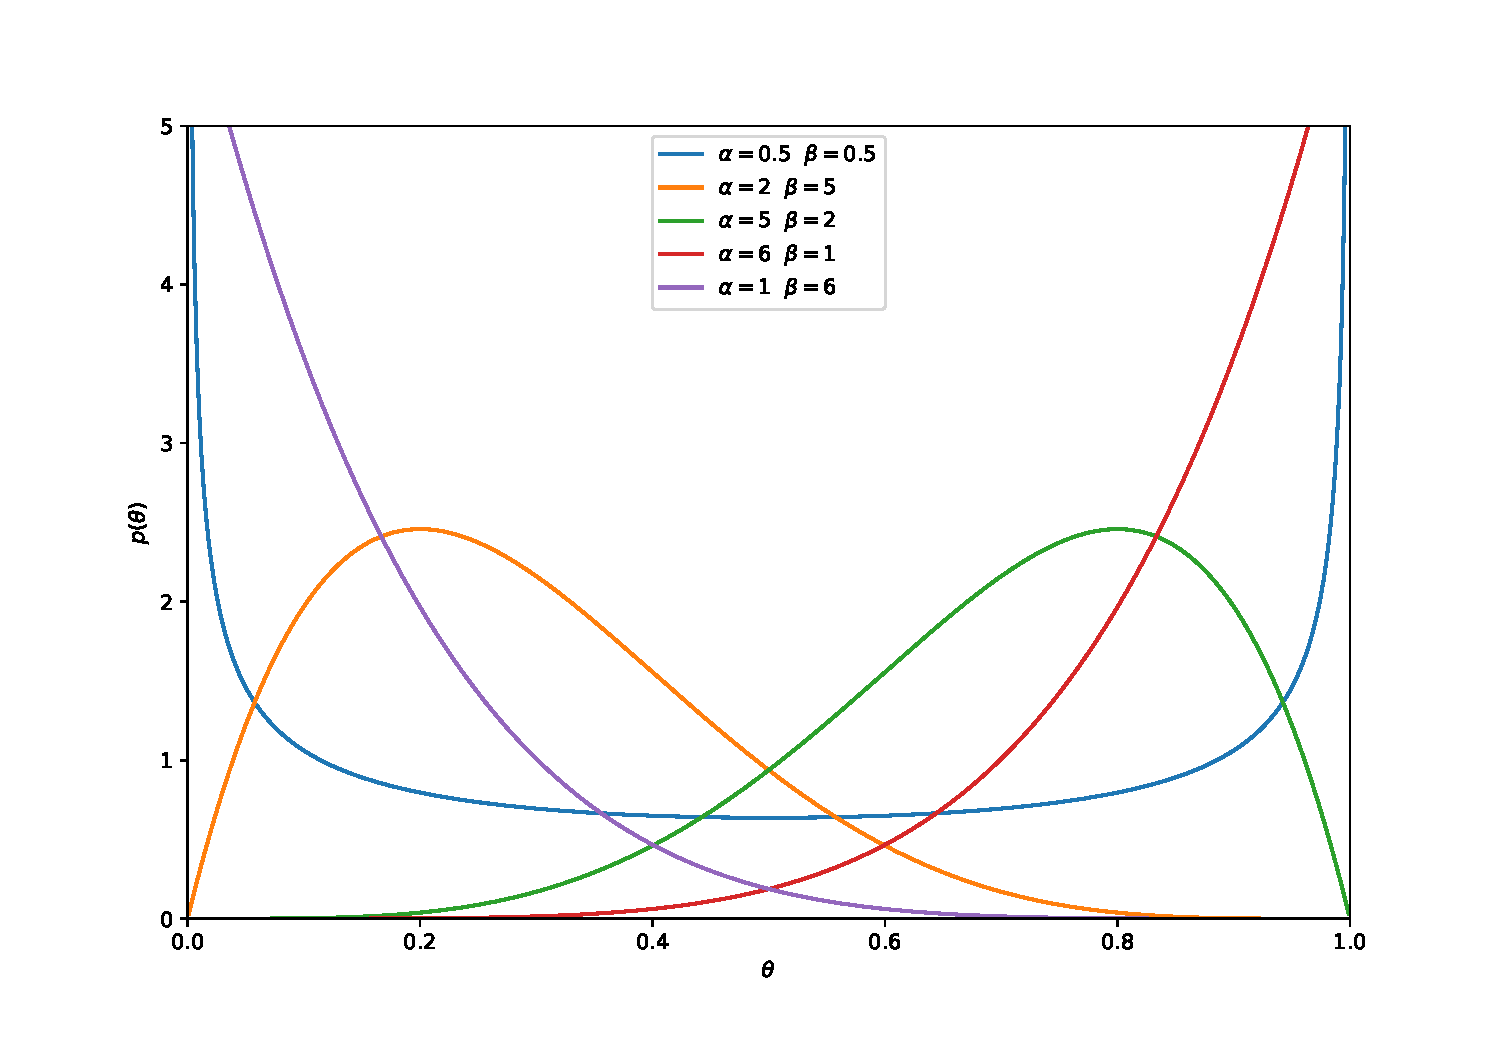
\includegraphics[width=0.55\textwidth, height=6cm]{img/cap2_beta.pdf}\\
	\caption{Elasticidad de la distribución beta de acuerdo a distintos parámetros. Se observa la interpretación del parámetro $\alpha$ como aciertos y $\beta$ como fracasos.}
\end{figure}


Adicionalmente, notemos que la magnitud de los parámetros va aumentando. La consecuencia de esto es que la varianza de la posterior va disminuyendo, pues 
\begin{equation}
	\V(\theta|\alpha,\beta) = \frac{\alpha\beta}{(\alpha+\beta)^2(\alpha+\beta+1)} \to 0 \text{ cuando }\alpha,\beta\to 0
\end{equation}
con lo que la incertidumbre de la distribución posterior de $\theta$ va disminuyendo a medida que vemos más observaciones. 



\begin{mdframed}[style=ejemplo, frametitle={\center Ejemplo: modelo binomial}]

Apliquemos la actualización bayesiana en el modelo binomial. Consideremos la variable binomial $k$ dada por
\begin{equation}
	k \sim \binom{n}{k}\theta^k(1-\theta)^{n-k},
\end{equation}
con probabilidad $\theta=0.66$ (desconocida). Nuestro objetivo es ver cómo depende la distribución posterior de $\theta$ de la elección del prior a medida que vamos obteniendo más observaciones. Para esto, elegimos 20 priors Beta distintos para $\theta$ dados por 
\begin{equation}
	p_i(\theta)  = \text{Beta}(\alpha_i,\beta_i),\  i=1,\ldots,20,
\end{equation}
donde $\alpha_i,\beta_i\sim U(1,10)$ (iid y discreto).

Ahora, realizaremos tres experimentos, en los cuales elegimos $n\in\{10,100,1000\}$ lanzamientos y calculamos los parámetros de las distribuciones a posteriori correspondientes a cada prior de acuerdo a las ecs.~\eqref{eq:bayes_update_bin1}-\eqref{eq:bayes_update_bin2}. En la Figura \ref{fig:bayes_binomial} podemos ver, desde izquierda a dercha, las  distribuciones a priori elegidas y luego las posteriores correspondientes a 10, 100 y 1000 observaciones. Notemos cómo a medida obtenemos más y más datos, la elección del prior es vuelve irrelevante y, como es de esperar, la evidencia de los datos es suficiente para aprender el modelo exitosamente (pues $\theta  =  0.66$) sin  depender del prior.

\begin{figure}[H] 
	\centering	
	\includegraphics[width=0.75\textwidth,frame ]{img/cap1_bayesian_binomial.pdf}
	\caption{Concentración de la distribución posterior en el modelo binomial.}
	\label{fig:bayes_binomial}
\end{figure}

\end{mdframed}


\subsubsection{Maximo a posteriori}
\label{sub:map}

Como ha sido el criterio en esta sección, mediante la distribución posterior podemos representar toda la información que nuestros sesgos y los datos aportan a la caracterización de un modelo (o parámetro), es decir, simetrías, barras de error, momentos, etc. En particular, es relevante verificar cómo podemos obtener estimaciones puntuales, en una forma similar a las obtenidas mediante mínimos cuadrados o máxima verosimilitud, a través del análisis de la distribución posterior. La motivación para la obtención de estimaciones puntales viene de i) la necesidad de comparar dichas estimaciones con las obtenidas por MC, MCR y MV, y además ii) los casos donde en efecto necesitamos una estimación puntual y no distribucional, como el problema de toma de decisiones.

Hay distintas alternativas evidentes para extraer una estimación puntual del parámetro $\theta$ desde la distribución $p(\theta|\datos)$, como la media, la mediana y la moda, las cuales son equivalentes cuando la posterior es  Gaussiana (o unimodal y simétrica en general). Siguiendo un criterio similar al de máxima verosimilitud consideraremos estimaciones puntuales mediante la maximización de la distribución posterior, consecuentemente, resumiendo la información de la posterior mediante su moda. 

\begin{definition}[Máximo a posteriori]
Sea $\theta\in\Theta$ un parámetro con distribución posterior $p(\theta|\datos)$ definida en todo $\Theta$, entonces nos referimos a estimación puntal dada por
\begin{equation}
	\thetaMAP = \argmax_{\Theta}p(\theta|\datos),
\end{equation}
como \emph{máximo a posteriori (MAP)}.

\end{definition}

Notemos que es posible encontrar el MAP incluso cuando solo tenemos acceso a una versión \emph{proporcional} a la distribución posterior, un escenario usual en inferencia bayesiana, o también mediante la maximización del logaritmo de ésta última. En efecto, 
\begin{equation}
	\thetaMAP = \argmax_{\theta\in\Theta}p(\theta|\datos) = \argmax_{\theta\in\Theta}p(\datos|\theta)p(\theta)= \argmax_{\theta\in\Theta}\left(\underbrace{\log p(\datos|\theta)}_{l(\theta)} + \log p(\theta)\right),
\end{equation}
donde  nuevamente vemos la maximización de  la función de log-verosimilitud, pero ahora junto al log-prior. Es evidente de esta expresión que si el prior no depende de $\theta$, es decir, si es uniforme, entonces el criterio MAP es equivalente al MV.

\begin{mdframed}[style=ejemplo, frametitle={\center Ejemplo: máximo a posterior para el modelo lineal y gaussiano}]
En particular, para el modelo lineal y gaussiano que hemos considerado hasta ahora, podemos calcular $\thetaMAP$ para un prior gaussiano multivariado donde cada coordenada de $\theta$ tendrá un prior independiente de media cero y varianza $\sigma_\theta^2$ (es decir, la matriz de covarianzas será diagonal). Asumiendo la varianza del ruido $\sigma_\epsilon^2$ conocida, se tiene que:	
\begin{align}
	\theta_\text{MAP}^\star 	&= \argmax_\theta p(Y|\tX,\theta)p(\theta)\nonumber\\
	&= \argmax_\theta \left(\prod_{i=1}^N \cN(y_i;\theta^\top\tx_i,\sigma_\epsilon^2)\right)\text{MVN}(\theta;0,\sigma_\theta^2\eye) \nonumber\\
	&= \argmax_\theta \left(\prod_{i=1}^N \frac{1}{\sqrt{2\pi}\sigma_\epsilon} \exp\left[{\frac{-1}{2\sigma_\epsilon^2}(y_i-\theta^\top\tx_i)^2}\right]\right)									\frac{1}{(\sqrt{2\pi}\sigma_\theta)^{M+1}} \exp\left({\frac{-\theta^\top\theta}{2\sigma_\theta^2}}\right) \nonumber\\
	&= \argmax_\theta  \frac{1}{(\sqrt{2\pi}\sigma_\epsilon)^N} \frac{1}{(\sqrt{2\pi}\sigma_\theta)^{M+1}} \exp\left( \sum_{i=1}^N{\frac{-1}{2\sigma_\epsilon^2}(y_i-\theta^\top\tx_i)^2} -{\frac{||\theta||^2}{2\sigma_\theta^2}}\right) \nonumber\\
	&= \argmin_\theta \sum_{i=1}^N{(y_i-\theta^\top\tx_i)^2} +{\frac{\sigma_\epsilon^2}{\sigma_\theta^2}||\theta||^2}.\label{eq:MAP_reg_lin}
\end{align}

Observemos que esta expresión es equivalente al costo cuadrático regularizado de la ec.~\eqref{eq:reg_least_squares} con orden $p=2$, es decir, la solución \emph{máximo a posteriori} del modelo lineal y Gaussiano con prior Gaussiano es equivalente a la de mínimos cuadrados regularizados (con orden de  regularización $p=2$). 

\end{mdframed}

Si bien en la ec.~\eqref{eq:MAP_reg_lin} elegimos un prior Gaussiano, pudimos haber elegido un prior exponencial $p(\theta)\propto\exp(\gamma|\theta|)$, con lo que habríamos llegado a MCR con regularización $p=1$ (o LASSO). Esto conecta claramente el uso de una distribución a priori dentro de la inferencia Bayesiana con el criterio general de regularización: El imponer un prior sobre $\theta$ es \emph{promover}, mediante probabilidades relativas, algunas soluciones para $\theta$; mientras que, por el contrario, el uso de un regularizador \emph{penaliza} algunas soluciones. Ajustando apropiadamente la función de regularización y la distribución a priori, podemos llegar a soluciones equivalentes en ambos casos, en particular, la elección de un prior uniforme equivale a un coeficiente de regularización $\rho$ nulo. Sin embargo, debemos recordar que además de la estimación puntual MAP, el enfoque bayesiano entrega la distribución completa sobre el parámetro desconocido. \\ 

Un ejemplo de la conexión entre regularizadores y priors puede ser obtenido directamente del desarrollo anterior. La razón entre las varianzas del ruido y del prior en la ec.~\eqref{eq:MAP_reg_lin}, dada por $\sigma_\epsilon^2/\sigma_\theta^2$, toma el mismo rol que el peso del regularizador $\rho/p$ en la formulación de MCR en la  ec.~\eqref{eq:reg_least_squares}. Esto implica que un prior con varianza $\sigma_\theta^2$ pequeña (cf. grande) es equivalente a un problema de MCR con un $\rho$ grande (cf. pequeño), lo cual tiene sentido:  $\theta$ puede ser ``llevado a cero'' mediante la asignación de un prior concentrado en cero o bien penalizando el magnitud de $\theta$ (MCR).\\

Desde ahora, podemos referirnos como MAP a las estimaciones puntuales en general pues, como acabamos de ver, ésta es equivalente a MCR y al mismo tiempo contiene al criterio de máxima verosimilitud como caso particular (cuando el prior es uniforme). Además, para modelos generales (distintos al caso lineal y gaussiano) el MAP no podrá ser calculado de forma explícita imponiendo 
\begin{equation}
 	\nabla_\theta  \log p(\theta|\datos) = 0,
 \end{equation}
 sino que tendremos que considerar algoritmos de optimización. En particular consideraremos algoritmos basados en derivadas con iteraciones de la forma
 \begin{equation}
 	\theta_{i+1} = \theta_i + \eta \nabla_\theta  \log p(\theta_i|\datos), \label{eq:itera_MAP_grad}
 \end{equation}
 donde esperamos que la secuencia $\{\theta_i\}_i$, al avanzar en el \emph{ascenso del gradiente de $\log p(\theta_i|\datos)$}, tienda al punto fijo de la ec.~\eqref{eq:itera_MAP_grad}, es decir, $\nabla_\theta  \log p(\theta|\datos) = 0$ (ver método del gradiente en anexos). 

\begin{remark} 
En el resto del curso, veremos distintos modelos que requieren técnicas sofisticadas de optimización, las cuales permiten no solo \emph{entrenar} dichos modelos (i.e., encontrar sus parámetros), sino también entender cómo funcionan; estos incluyen redes neuronales,  máquinas de soporte vectorial y procesos gaussianos. Con lo visto hasta ahora podemos ver que el aprendizaje de máquinas, se sustenta  en dos elementos fundamentales: el modelamiento probabilístico que permite definir \emph{posibles} modelos, y el proceso de optimización que permite encontrar el \emph{buen modelo}. Podemos entonces, a \emph{grosso modo}, decir que ``aprender es optimizar''.
\end{remark}


\begin{mdframed}[style=ejemplo, frametitle={\center Ejemplo: MAP para el modelo binomial}]

Siguiendo el ejemplo anterior de la distribución binomial, recordemos que al asumir un prior $p(\theta) = \text{Beta}\left(\theta; \alpha,\beta \right)$ para el parámetro $\theta$, la posterior del mismo (dado un conjuntos de $N$ experimentos con $\{n_i\}$ lanzamientos  y $\{k\}_i$ aciertos) está dada por 
\begin{equation}
  	\text{Beta}\left(\theta; \alpha + \sum_{i=1}^N k_i, \beta + \sum_{i=1}^N n_i - k_i \right).
  \end{equation}
  Denotando los parámetros de la posterior mediante $\alpha_N = \alpha + \sum_{i=1}^N k_i$ y $\beta_N = \beta + \sum_{i=1}^N n_i-k_i$, podemos encontrar el MAP mediante
  \begin{align}
  	\thetaMAP &= \argmax \theta^{\alpha_N - 1}(1-\theta)^{\beta_N -1} = \frac{\alpha_N - 1}{\alpha_N + \beta_N - 2,
  	}\nonumber
  \end{align}
  pues el cálculo no es necesario ya que la moda de la distribución Beta es conocida. Además, la varianza posterior, está dada por 
  \begin{equation}
  	\V[\theta|\datos] = \frac{\alpha_N \beta_N }{(\alpha_N  + \alpha_N )^2(\alpha_N  + \beta_N +1)}.
  \end{equation}
  Es directo ver que, como función de las sumas de aciertos/fallos, cuando  observamos muchos datos $\thetaMAP$ tiende a la razón entre aciertos y lanzamientos  totales y $\V[\theta|\datos] $ tiende a cero. Verificaremos esto numéricamente de la misma forma que el ejemplo anterior: consideremos 20 priors Beta con parámetros $\alpha$ y $\beta$ aleatorios entre 1 y 10 y grafiquemos tanto $\thetaMAP$ como $\V[\theta|\datos] $ en función de un númeo creciente de lanzamientos binomiales. La Figura \ref{fig:binomial_MAP} confirma nuestra intuición donde (con escala logarítmica para el eje $x$) podemos ver que con 10 lanzamientos, ya se ve una clara tendencia, mientras que con 100 lanzamientos la convergencia es indudable. 

\begin{figure}[H]
	\centering
	\includegraphics[width=0.9\textwidth]{img/cap1_bayesian_binomial_MAP.pdf}
	\caption{Concentración de MAP y reducción de varianza posterior: modelo binomial.}
	\label{fig:binomial_MAP}
\end{figure}


\end{mdframed}

\subsection{Predicciones}
\label{sub:predicciones}

Luego de haber discutido la estimación de parámetros, tanto desde el punto de vista puntual (MC, MCR, MV, MAP) como de estimación bayesiana, ahora veremos cómo estas estimaciones se utilizan para hacer predicciones. \\

Definamos en primer lugar el contexto para nuestra pedicción. Consideremos un modelo $p(y|x)$, con parámetro $\theta$, del cual se han obtenido datos denotados mediante $\datos = \{(x_i,y_i)\}_{i=1}^N$. Además, introduciremos el concepto de \emph{variable latente}, es decir, una variable dentro del modelo que no es observable, pero que nos interesa predecir. Esta definición es clave para estudiar la predicción: si bien la construcción del modelo para $y$ tiene como objetivo modelar la generación de datos ($\theta$) y sus observaciones ($\sigma$), nuestro objetivo final es predecir la cantidad latente, no la observación futura;  pues la observación contiene una perturbación asociada a su incertidumbre aleatoria. En el caso lineal, por ejemplo, denotamos la variable latente como $f = \theta^\top x$, donde el modelo está dado por
\begin{equation}
		 y = \theta^\top x  + \epsilon = f + \epsilon, \quad \epsilon \sim \cN(0,\sigma^2).
\end{equation}
Denotaremos entonces mediante $\hat f_\star$ e $\hat y_\star$ las predicciones de la variable latente $f$ y la observación $y$ para una nueva entrada $x_\star$, condicional a los datos observados $\datos$. A continuación veremos que distintos supuestos sobre la estimación de $\theta$ resultan en distintas predicciones para estas cantidades, donde utilizaremos el modelo lineal/gaussiano de varianza conocida para ilustrar estas diferencias. 

En primer lugar consideremos las estimaciones puntuales, en cuyo caso realizamos un procedimiento conocido como \emph{plug-in prediction}, en donde simplemente utilizamos el valor (puntual) la estimación del parámetro dentro del modelo. En el ejemplo del modelo lineal, si hemos calculado el parámetro mediante máxima verosimilitud (denotado como $\theta_{\text{MV}}$) entonces nuestro modelo lineal estimado es $y = \theta_{\text{MV}}^\top \tilde{x} + \epsilon$. Con lo que la predicción usual de la variable lantente correspondiente a una entrada $\tilde{x}_\star$ es determinista (pues tanto $\theta_{\text{MV}}$ como $x_\star$ lo son) y dada por
\begin{equation}
	\hat f_\star = \theta_{\text{MV}}^\top \tilde{x}_\star.
\end{equation}
Por el contrario, si lo que quisiésemos estimar es efectivamente la variable aleatoria $y_\star|\tilde{x}_\star$ (la cual incluye el ruido de observación), esta predicción está dada por 
\begin{equation}
	\hat y_\star \sim \cN(\theta_{\text{MV}}^\top \tilde{x}_\star,\sigma^2). 
\end{equation}
Gráficamente, es también usual representar esta predicción en términos de su esperanza y \emph{barras de error}, las cuales para el caso gaussiano son explícitas para el 95\% en función de la desviación estándar del ruido $\epsilon$. Es decir, con un 95\% de probabilidad, $\hat y_\star\in[\theta_{\text{MV}}^\top \tilde{x}_\star - 2\sigma,\theta_{\text{MV}}^\top \tilde{x}_\star + 2\sigma]$. \\

A diferencia de las estimaciones puntuales, cuando el parámetro $\theta$ es estimado de forma bayesiana (disponemos de su distribución posterior) el modelo estimado en sí es una \textbf{distribución aleatoria} pues el modelo es una función determinista de un parámetro $\theta$ aleatorio. Podemos entonces identificar dos fuentes de incertidumbre en el modelo aprendido como discutimos al comienzo de esta sección: la epistemológica dada por la distribución posterior de $\theta$, y la aleatoria dada por la distribución de $\epsilon$. En nuestro ejemplo del modelo lineal y Gaussiano con varianza conocida el modelo aprendido está dado por
\begin{equation}
		 y = \theta^\top \tilde{x} + \epsilon, \quad \epsilon \sim \cN(0,\sigma^2),\ \theta \sim p(\theta|\datos) = \cN(\theta_N,\sigma^2\Lambda_n^{-1}),
\end{equation}
donde los parámetros de la posterior de $\theta$ están descritos en las ecs.~\eqref{eq:mean_post_lin_g}-\eqref{eq:var_post_lin_g}. Podemos ver entonces que la relación que tenemos para $y$ está \emph{amarrada} a otras cantidades aleatorias ($\theta$ y $\epsilon$), de las cuales nos debemos deshacer para producir la predicción. Esto es porque la introducción de dichas variables fue necesaria para aprender la relación entre $x$ e $y$ a través de nuestro modelo propuesto (o supuesto), y no tienen \emph{necesariamente alguna relación con la realidad}. En la literatura clásica, estos parámetros son llamados \emph{nuisance parameters} y su remoción, la cual es realizda a través del cálculo de una integral, es referido como \emph{to integrate out}. Es difícil acordar una traducción al español de este concepto, el cual automáticamente suguiere que estamos ``sacando'' (\emph{out}) estos parámetros mediante integración; a falta de un mejor término simplemente usaremos la expresión en inglés o su desafortunada traducción ``desintegrar''. Por lo tanto, la distribución posterior de la variable latente  está dada por la ``desintegración'' de $\theta$  con respecto a su propia distribución posterior, es decir,
\begin{equation}
	\hat f_\star \sim p(f_\star|x_\star,\datos) = \int p(f_\star, \theta|x_\star,\datos)\d\theta = \int p(f_\star|x_\star, \datos, \theta)p( \theta|\datos,x_\star)\d\theta= \int p(f_\star|x_\star, \theta)p( \theta|\datos)\d\theta\label{eq:integrate_out_pred}
\end{equation}
donde, de izquierda a derecha: 
\begin{itemize}
	\item la primera igualdad pretende \emph{hacer aparecer} $p(f|\theta)$ que es lo que realmente conocemos, donde $p(f|\datos)$ va a ser calculado mediante la desintegración de $\theta$
	\item la segunda igualdad es simplemente la definición de distribución condicional
	\item la tercera igualdad elimina redundacias: dado $\theta$ y $x_\star$, $f_\star$ no depende de los datos; de igual forma, la distribución posterior del parámetro depende solo de los datos pasados, no de un nuevo input ya que $x_\star$ no aporta información (no se conoce su salida).
\end{itemize}
En el caso lineal/gaussiano, el integrando de la expresión más a la derecha de la eq.~\eqref{eq:integrate_out_pred} es la multiplicación de dos gaussianas. Si bien el cálculo de dicha integral es tedioso, ésta tiene la forma de una convolución entre dos gaussianas y sabemos\footnote{Verificable fácilmente a través del teorema de la convolución.} que eso resulta en, nuevamente, una gaussiana. En el caso lineal, sin embargo, ni siquiera es necesario calcular dicha integral, pues podemos calcular la ley posterior de $f_\star$ notando simplemente que $f = \theta^\top \tilde{x}_\star$ y que $\theta \sim \cN(\theta_N,\sigma^2\Lambda_n^{-1})$, lo cual da por linealidad:
\begin{equation}
	\hat f_\star \sim p(f_\star|x_\star,\datos) = \cN(\theta_N^\top \tilde{x}_\star,\tilde{x}_\star^\top\sigma^2\Lambda_n^{-1} \tilde{x}_\star).\label{eq:post_pref_f}
\end{equation}
Desde esta expresión es posible graficar el modelo mediante la determinación de las barras de error de los parámetros o bien generando una muestra para el parámetro desde su distribución posterior y luego graficar el modelo con dicha muestra --- esto es equivalente a samplear desde la posterior del modelo.\\

Finalmente, para determinar la predicción de la observación ruidosa $y=f+\epsilon$, simplemente notemos que esta estará dada por la incorporación del estadístico del ruido a la expresión en eq.~\eqref{eq:post_pref_f}, en efecto,
\begin{equation}
	\hat y_\star\sim\cN(\theta_N^\top \tilde{x}_\star,\tilde{x}_\star^\top\sigma^2\Lambda_n^{-1} \tilde{x}_\star + \sigma^2).
\end{equation}

\begin{remark}\label{rem:predicciones}
De la predicción bayesiana en forma de distribución de la ec.~\eqref{eq:post_pref_f} podemos obtener (y es usualmente necesario) una predicción puntual dada por la media, la cual corresponde a 
\begin{equation}
	\E[f_\star|x_\star,\datos] = \E[\theta|\datos]^\top  \tilde{x}_\star = \bar \theta^\top  \tilde{x}_\star, 
\end{equation}
donde hemos denotado por $\bar \theta$ a la media posterior de $\theta$. Consecuentemente, las estimaciones puntuales reportadas por el método bayesiano y de estimación puntual resultan en la misma predicción. Este fenómeno solo ocurre en situaciones particular, en este caso, debido a que el modelo es lineal y gaussiano. 
\end{remark}

Finalmente, la Fig.~\ref{fig:rpredicciones_reg_lin} muestra la implementación de las 4 formas de predecir usando el modelo lineal aplicado al dataset de grillos y temperatura usado inicialmente en la Fig.~\ref{fig:reg_lin_reg}. Es posible ver como la  predicción bayesiana da sutilmente distintas predicciones que en los extremos del modelo reportan más incertidumbre, mientras que la predicción de $y$ considera tanto ruido que presenta una banda de incertidumbre \emph{uniforme} a lo largo de las observaciones. 
\begin{figure}[H]
	\centering
	\includegraphics[width=0.45\textwidth]{img/cap1_chirridos_pred1}
	\includegraphics[width=0.45\textwidth]{img/cap1_chirridos_pred2}
	\includegraphics[width=0.45\textwidth]{img/cap1_chirridos_pred3}
	\includegraphics[width=0.45\textwidth]{img/cap1_chirridos_pred4}
	\caption{Ejemplo de predicción usando el modelo lineal para la  base de datos de grillos y temperatura. Desde la esquina superior izquierda: predicción plug-in de $f$, predicción plug-in de $y$, predicción bayesiana de $f$ (20 muestras), predicción bayesiana de $y$ (20 muestras).}
	\label{fig:rpredicciones_reg_lin} 
\end{figure}

\subsection{Regresión no lineal}

El modelo de regresión lineal visto en las secciones anteriores tiene diversas ventajas, en primer lugar su solución en el caso de mínimos cuadrados (o máxima verosimilitud en el caso de ruido gaussiano) puede ser encontrado de forma explícita y única. Además, sus parámetros permiten interpretar la relación entre cada una de las componentes de la variable de entrada y la variable de salida. Sin embargo, más allá de estas propiedades del modelo lineal, su alcance es muy limitado pues muchas veces necesitamos modelar fenómenos que no siguen una relación lineal. \\

El concepto de regresión lineal puede ser extendido a una contraparte no lineal en los casos particulares que conocemos a priori el tipo de relación entre las variables de entrada $x$ y salida $y$ (y esta  no es lineal). Dicha extensión puede ser obtenida simplemente mediante la aplicación de una transformación (de parámetros fijos) a la variable independiente, e.g. $\phi(x)$, para luego construir un modelo lineal en la variable transformada $\phi=\phi(x)$ en lugar de en la variable original $x$. 

Específicamente, consideraremos transformaciones a valores vectoriales de la variable independiente de la siguiente forma
\begin{align}
  \phi \colon \R^M &\to \R^D \nonumber\\
  x &\mapsto \phi(x)=[\phi_1(x),\ldots,\phi_D(x)]^\top,
\end{align}
donde $\phi_i: x\in\R^M \mapsto \phi_i(x)\in\R$ son funciones escalares $\forall i=1,\ldots,D$.\\

Con la introducción de la transformación $\phi(\cdot)$ es necesario hacer la distinción entre ambas variables de entrada. Nos referiremos entonces a $x$ como datos/entradas crudos (\emph{raw data/input}) y a la variable  $\phi=\phi(x)$ como  características (\emph{features}). Recordemos que los modelos del capítulo anterior eran aplicados directamente sobre la entrada cruda $x$ (o $\tilde{x}$), con lo que no existía distinción entre entradas crudas o características. Adicionalmente, la introducción  del concepto de \emph{característica} es motivado por la búsqueda de una representación de $x$ que permite resolver el problema de regresión usando un modelo simple (y también interpretable) como el modelo lineal, a diferencia de la idea de diseñar un modelo muy complicado (no interpretable) que reciba directamente la entrada cruda $x$. Un ejemplo de esto es el caso en que $x$ es una imagen: en este caso no es posible aplicar directamente un modelo lineal a la representación matricial de la imagen, sino que a una representación distinta de esta, o a sus \emph{características}, es decir, sus bordes, formas, y otros patrones a identificar dentro de la imagen.\\

En la práctica, la función $\phi:x\mapsto\phi(x)$ es elegida en base  al conocimiento \emph{experto} que se tenga del problema de regresión a resolver;  como su elección pretende extraer las características de interés y representarlas  de una forma compatible con el modelo lineal, entonces, nos referiremos a la construcción \emph{manual} de la función $\phi$ como \emph{ingeniería de características}. Observemos entonces que la función $\phi$ puede tener (y en general tiene) parámetros, los cuales en esta primera instancia serán elegidos manualmente. Sin embargo, más adelante veremos modelos donde los parámetros de $\phi$ también pueden ser encontrados de forma automática (e.g., mediante máxima verosimilitud). En dicho caso, es posible interpretar que la ingeniería de características ya no es realizada de forma manual, sino que automatizada.  


\begin{mdframed}[style=discusion, frametitle={\center Características y modelos}]
El diseño de características es uno de los problemas fundamentales del AM. Esto porque podemos entender la construcción de modelos de aprendizaje supervisado como dos etapas: i) la identificación de las características relevantes y ii) cómo usar estas características para estimar el output (el modelo). En el modelo no lineal presentado aquí, es claro que la parte no lineal $\phi$ es la característica y la parte lineal es el modelo, sin embargo, en el caso general la línea entre ambas etapas es muy delgada.  Por ejemplo, en una red neuronal de 100 capas, ¿qué corresponde a característica y qué corresponde al modelo? Podríamos argumentar que en modelos más complicados como los de redes neuronales, existen varias interpretaciones de qué corresponde a cada cosa, y con eso de paso interpretar qué está haciendo nuestro modelo. El hecho de que el diseño de características y el modelo se confundan es interesante también, pues quiere decir que las características se aprenden de igual forma que el resto del modelo; con lo que pasamos desde un diseño manual de características a una búsqueda automáticas de características. 

\end{mdframed}


\subsubsection{Modelo lineal en los parámetros} 
\label{sub:modelo_lineal_param}


Usando la nueva variable de  características $\phi=\phi(x)$ como entrada a un modelo lineal, podemos definir el siguiente modelo de regresión lineal y gaussiano: 
\begin{equation}
    y = \theta^\top\phi(x) + \epsilon,\quad \epsilon\sim\cN(0,\sigma_\epsilon^2)\label{eq:reg_no_lin},
\end{equation}
donde asumiremos que contamos con un conjunto de observaciones de la forma
\begin{equation}
    \datos = \{(x_i,y_i)\}_{i=1}^N,\quad (x_i, y_i)\in\R^M\times\R,\forall i=1,\ldots,N.
    \label{eq:training_set_nl}
\end{equation}

De la misma forma que vimos en el capítulo anterior, este modelo puede ser entrenado mediante la optimización de costo cuadrático:
\begin{equation}
	J = \sum_{i=1}^N(y_i - \theta^\top\phi(x_i))^2
	\end{equation}

lo cual es equivalente a máxima verosimilitud, pues el ruido de observación $\epsilon$ es gaussiano.\\

Además, se puede compactar el funcional utilizando la matriz de diseño al igual que en regresión lineal:

\begin{align}
    \Phi = 
    \left[ \begin{matrix} \phi(x_1)^\top\\
    \vdots \\
    \phi(x_N)^\top\\
    \end{matrix} \right]
     = \left[ \begin{matrix} \phi_1(x_1)& \ldots & \phi_D(x_1)\\
    \vdots & \ddots & \vdots \\
    \phi_1(x_N) & \ldots & \phi_D(x_N)\\
    \end{matrix} \right]
    \qquad
    Y = \left[ \begin{matrix} y_1 \\ \vdots \\ y_N \end{matrix} \right],
\end{align}
con lo que el modelo y el funcional de costo puede ser expresados respectivamente mediante
\begin{align}
    Y &= \Phi\theta + \bepsilon,\quad \bepsilon\sim\cN(\mathbf{0},\sigma_\epsilon^2\mathbf{I})\\
    J &= (Y-\Phi\theta)^\top(Y-\Phi\theta) = \norm{Y-\Phi\theta}_2^2
\end{align}

De forma análoga al modelo lineal estándar (el cual toma directamente la variable cruda $x$ como input), la minimización del funcional $J$ puede  ser encontrado mediante la condición de primer orden $\nabla_\theta J=0$ ya que el costo es estrictamente convexo. De este modo:
\begin{align}
    \theta{\star}&= (\Phi^\top\Phi)^{-1}\Phi^\top Y\label{eq:nolin_theta}.
\end{align}
Las siguientes observaciones conectan el modelo no lineal de la ec.~\eqref{eq:reg_no_lin} con el modelo lineal estudiado en las secciones anteriores.


\begin{remark}
De la ec.~\eqref{eq:nolin_theta} vemos que si elegimos $\phi(\cdot) = \text{id}(\cdot)$ recuperamos la expresión para mínimos cuadrados ordinarios. Esto permite interpretar el modelo de regresión no lineal con variables $\{(x_i,y_i)\}_{i=1}^N$ de $\R^N$ a $\R$ como una regresión lineal con variables $\{(\Phi(x_i),y_i)\}_{i=1}^N$ de $\R^D$ a $\R$. Además, la razón por la que la forma de la solución es la misma que el caso lineal es porque si bien el modelo presentado en la ec.~\eqref{eq:reg_no_lin} es no  lineal en la entrada $x$, este sí es \emph{lineal en los parámetros} $\theta$.
\end{remark}

\begin{remark}
Notemos que la re-parametrización del modelo afín introducida en el capítulo anterior es un caso particular de la transformación $\Phi$. Esto es directo de la siguiente construcción:
\begin{align}
    \Phi &= [x, 1]^\top\\
    y &= a^\top x + b  =  \theta^\top\Phi(x)+ \epsilon.
\end{align}
\end{remark}


\begin{remark}
    Finalmente, es posible considerar una extensión regularizada al modelo no lineal presentado en la   ec.~\eqref{eq:reg_no_lin} mediante la consideración de un costo regularizado cuadrático (i.e., \emph{ridge regression}) dado por 
\begin{equation}
    J_\rho = \norm{Y-\Phi\theta}_2^2 + \rho\left \| \theta \right \|^2,\quad \rho\in\R^+.
\end{equation}
En cuyo caso, la solución está dada por
\begin{equation}
    \theta = (\Phi^\top\Phi+\rho\mathbb{I})^{-1}\Phi^\top Y.
\end{equation}
\end{remark}


\begin{mdframed}[style=discusion, frametitle={\center Selección de características}]

Un buen conjunto de características no solo ayuda a una buena representación (y consecuentemente predicción) de nuestros datos, sino que extrae literalmente las  \emph{características} que son relevantes de $x$ para determinar $y$. Por ejemplo, si necesitamos determinar la condición clínica de un  paciente, para el cual tenemos una vasta colección de  mediciones como peso, edad, género, dirección, número de teléfono, ocupación, color de ojos, salario, etc, muy probablemente muchas estas características no van a ser útil (por ejemplo, ocupación), con lo que el diseño de las funciones $\phi$ debe tomar en cuenta esto. Por el contrario, si necesitamos evaluar el mismo conjunto de individuos  para un crédito de consumo, las características a considerar variarán y ahora probablemente el salario sí juegue un rol importante. Este concepto permite entender la estrecha relación entre el diseño de características y la \emph{selección de características} y consecuentemente la \emph{selección de modelos}, lo cual veremos en los siguientes capítulos. En particular, recordemos que usando el regulador LASSO, podemos llevar algunas de nuestras coordenadas a cero, realizando una selección automática de características. 

\end{mdframed}


\subsubsection{Ejemplos de transformaciones}

La selección de las características es fundamental para una representación apropiada de nuestros datos y consecuentemente para el desempeño del modelo de regresión no lineal. En efecto, si la familia de funciones $\phi_1,\ldots,\phi_D$ no captura la representación de las características de forma compatible con el modelo lineal, el esfuerzo por ajustar la parte lineal del modelo será infructuoso. En general, la elección de la base de funciones debe ser diseñada y evaluada caso a caso.\\

A continuación vemos algunos ejemplos de características que son usualmente usadas en la práctica por su generalidad (habilidad para replicar varios comportamientos) y/o simpleza.\\

\noindent\textbf{Función Polinomial:} $\phi=\{\phi_i\}_{i=0}^D$, donde $\phi_i(x)=x^i$, de tal forma que 
\begin{equation}
    \Phi = \left[ \begin{matrix} 1 & x_1 & x_1^2 & \ldots & x_1^D\\
    \vdots & \vdots & \vdots & \ddots & \vdots \\
    1 & x_N & x_N^2 & \ldots & x_N^D\\
    \end{matrix} \right].
\end{equation}

La función polinomial es ampliamente usada ya que de acuerdo al teorema de Stone-Weierstrass, los polinomios son densos en $\mathcal{C}([a,b])$ (funciones continuas sobre compactos), por lo que es posible aproximar cualquier función continua mediante un polinomio, donde la precisión puede ser tan pequeña como se necesite. Sin embargo, una desventaja de esta  base es que tanto su entrenamiento como  predicciones pueden ser inestables: para obtener una buena aproximación polinomial, generalmente se requiere un grado $D$  alto, por lo que los valores de $\phi(x)$ crecen, obviamente, de forma \emph{polinomial}.\\

Por otra parte, la interpolación polinomial sufre del fenómeno de Runge, por lo que al utilizar un grado elevado, es posible que el error de predicción en los bordes crezca indefinidamente.\\

\noindent\textbf{Función Sinusoidal:} $\phi=\{\phi_i\}_{i=0}^D$, donde $\phi_i(x)=\cos\left(i\frac{2\pi}{2T}(x - b_i)\right)$. La variable $i$ actúa como una frecuencia normalizada con respecto al período de oscilación $T$ y $b_i$ es un ``offset''  o fase. Esta transformación está dada por
\begin{equation}
    \Phi = \left[ \begin{matrix}
    1 & \cos\left(1\frac{2\pi}{2T}(x_1-b_1)\right) & \ldots & \cos\left(D\frac{2\pi}{2T}(x_1-b_D)\right)\\
    \vdots & \vdots  & \ddots & \vdots \\
    1 & \cos\left(1\frac{2\pi}{2T}(x_N-b_1)\right) & \ldots & \cos\left(D\frac{2\pi}{2T}(x_N-b_D)\right)\\
    \end{matrix} \right].
\end{equation}
Hemos asumido que el la fase para cada función $\phi_i$, la frecuencia $i\frac{2\pi}{2T}$ y fase $b_i$ son fijas. Una forma de evitar definir una fase, es considerar dos transformaciones por cada $\phi_i$ de la forma
\begin{equation}
    \phi_i'(x) = \left[\sin\left(i\frac{2\pi}{2T}x\right),\ \cos\left(i\frac{2\pi}{2T}x\right)\right],
\end{equation}
donde no es necesario definir la fase sino que ésta es absorbida por el parámetro $\theta$ y aprendida.\\

Al igual que los polinomios, la base de senos y cosenos es también \emph{universal} (más aún, forman una base de Hilbert de $L^2$ en el círculo). Sin embargo, una desventaja de la base senoidal es que solo puede replicar funciones periódicas, con un período máximo en este caso  de $T$. En la práctica, veremos que un modelo sinusoidal se repetirá cada período, pudiendo llevar a conclusiones erróneas. Además, si efectivamente nuestros datos representan un comportamiento periódico pero el ruido de observación resulta en que cada período o \emph{forma de onda} sean ligeramente distinto, puede ser difícil encontrar el período $T$. La identificación de este período es un desafío en sí mismo, conocido como \emph{detección de periodicidades o frecuencias fundamentales}, usual en astronomía y procesamiento de audio. \\

\noindent\textbf{Funciones constantes por partes:} La siguiente característica está está compuesta por ``escalones'', los cuales valen ``1'' dentro de un conjunto especifico y ``0'' en cualquier otro lugar. Sean $c_1,c_2, \ldots,c_D\in\R$ una colección de valores crecientes, definimos la indicatriz $I_A$ y las funciones de pertenencia $C_i$:
\begin{align}
    C_0(x) &= I_{(-\infty,c_1)}(x)\\
    C_i(x) &= I_{[c_i,c_{i+1})}(x), \quad \forall i=1,\ldots,D-1\\
    C_D(x) &= I_{[c_D,+\infty)}(x)\\
    I_A(x) &= \left\{\begin{matrix}
    1,\quad x\in A\\
    0,\quad x\notin A
    \end{matrix}\right. 
\end{align}
De esta forma la base de funciones $\Phi=\{\phi_i\}_{i=0}^D$ queda definida por
    
\begin{align}
    \phi_i(x) &= C_i(x),\quad \forall i=0,\ldots,D\\
    \Phi(X) &= \left[ \begin{matrix}
    1 & C_0(x_1) & \ldots & C_D(x_1)\\
    \vdots & \vdots  & \ddots & \vdots \\
    1 & C_0(x_N) & \ldots & C_D(x_N)\\
    \end{matrix} \right].
\end{align}
Las funciones contantes por partes son útiles cuando trabajamos con experimentos que involucran una discretización, por ejemplo, al modelar la altura/concentración/conductividad/temperatura en una superficie y no es posible parametrizar esta cantidad como función del (en este caso) espacio. Entonces, simplemente dividimos la superficie en una grilla y asignamos un valor distinto a cada celda de esta grilla. Es un método útil pero la cantidad de parámetros (dimensión de $\theta$) crece con el número de celdas de la grilla, lo cual es prohibitivo para casos donde el  rango de valores de $x$ y/o su dimensión es medianamente alta. 
    
\iffalse
\noindent\textbf{Polinomios por partes (Splines)}: Una generalización de las funciones constantes por partes es ajustar polinomios truncados definidos en intervalos. Es decir, podríamos considerar el siguiente modelo truncado (dos partes solamente) 
\begin{equation}
    y = \left\{\begin{matrix}
    \beta_{01}+\beta_{11}x+\beta_{21}x^2+\beta_{31}x^3+\epsilon,\quad x < c\\
    \beta_{02}+\beta_{12}x+\beta_{22}x^2+\beta_{32}x^3+\epsilon,\quad x \geq c
    \end{matrix}\right.
\end{equation}
    
El problema con esta formulación es que en el punto $c$ no existe ninguna restricción de continuidad, lo cual es muchas veces necesario para que el modelo tenga sentido y refleje la realidad. Podemos arreglar esta discontinuidad de la siguiente forma.

Consideremos una secuencia de puntos crecientes $\xi_1,\ldots,\xi_K$ que serán los puntos en que cambia el régimen del polinomio, estos puntos se conocen como \emph{nudos}; en el ejemplo anterior solo consideramos un nudo para ilustrar. Podemos ahora definir el un polinomio truncado de grado $i$ con un nudo en $\xi_k$ mediante
\begin{equation}
    (x-\xi_k)_+^i = \left\{\begin{matrix}
    0,\quad x < \xi_k\\
    (x-\xi_k)^i,\quad x \geq \xi_k
    \end{matrix}\right.
\end{equation}
Con esto polinomio truncado de grado $D$ y con $K$ nudos queda definido por
    
    \begin{equation}
        y = \beta_0 + \sum_{d=1}^D\beta_dx^d+\sum_{k=1}^K(x-\xi_k)_+^D
    \end{equation}
    
    \begin{equation}
        \Phi(X) = \left[ \begin{matrix} 1 & x_1 & x_1^2 & \ldots & x_1^D & \ldots & (x_1-\xi_1)_+^D & \ldots & (x_1-\xi_K)_+^D \\
        \vdots & \vdots & \vdots & \ddots & \vdots & \ddots & \vdots & \ddots & \vdots\\
        1 & x_N & x_N^2 & \ldots & x_N^D & \ldots & (x_N-\xi_1)_+^D & \ldots & (x_N-\xi_K)_+^D \\
        \end{matrix} \right]
    \end{equation}

\fi


\begin{mdframed}[style=ejemplo, frametitle={\center Ejemplo: Predicción de pasajeros de una aerolínea)}]

Consideremos el problema de predecir la cantidad de pasajeros en una aerolínea, considerando  distintas combinaciones de características. De forma incremental, tomaremos en consideración características polinomiales,  senoidales, y senoidales con amplitud creciente. Es decir, denotando $x$ en tiempo y $y$  la cantidad de pasajero, consideraremos el siguiente modelo
\begin{equation}
    y = \underbrace{\sum_{i=0}^3 \theta_i x^i}_\text{parte polinomial} + \underbrace{ \sum_{i=1}^2 \alpha_i\exp(-\tau_ix^2)\cos(\omega_i(x-\psi_i))}_\text{parte oscilatoria}.
\end{equation}
La motivación de este modelo es representar la tendencia de los datos mediante la componente polinomial y la oscilación anual mediante las componentes oscilatorias.

Además, hemos considerado 12 años de datos con frecuencia mensual (144 datos), de los cuales solo 9 años (108 datos) han sido usado para encontrar los parámetros del modelo y los  3 años restantes (36 datos) para validar nuestras predicciones. La Figura \ref{fig:pasajeros} muestra los datos y las estimaciones para 3 variantes del modelo mencionado: parte polinomial, parte polinomial y oscilatoria de amplitud fija, y finalmente,  parte polinomial y oscilatoria de amplitud variable. En cada gráfico se muestran distintas opciones de cada  modelo en gris con la mejor  trayectoria en negro; se puede ver además en cada gráfico cómo disminuye el error de aproximación a medida consideramos más características. 


\begin{figure}[H]
    \centering
    \includegraphics[width=0.9\textwidth, frame]{img/cap1_pasajeros.pdf}
    \caption{Regresión no-linea de cantidad de pasajeros en el tiempo. Arriba-izq: datos de entrenamiento, arriba-der: modelo con componente polinomial, abajo-izq: modelo con componentes polinomial y oscilatoria (amplitud fija), abajo-der: modelo con componentes polinomial y oscilatoria (amplitud creciente).}
    \label{fig:pasajeros}  
\end{figure}
\end{mdframed}

\subsection{Árboles}
